%Kompiliuoti su XeLaTeX ir BibTeX

\documentclass[a4paper, 12pt, oneside]{article}

\usepackage[yyyymmdd]{datetime}

\usepackage{fontspec}
\usepackage{fontenc}
\usepackage{ulem}
\usepackage{cite}
\usepackage{mathtools}
\usepackage{amsmath}
\usepackage{amssymb}
%\usepackage{float}
\usepackage{graphicx}
\usepackage{multirow}
\usepackage[hyphens]{url}
\usepackage{caption}
\usepackage[svgnames]{xcolor}
\usepackage{lineno}
\usepackage[lithuanian]{babel}
\usepackage{hyperref}
\usepackage{siunitx}
\usepackage{floatrow}
\usepackage{indentfirst}
%\usepackage[parfill]{parskip}

\floatsetup[table]{capposition=top}

\hypersetup{breaklinks=true}
\urlstyle{same}

\usepackage{geometry}
\pagestyle{myheadings}
\geometry{
	left=3cm,
	right=1cm,
	top=2cm,
	bottom=2cm,
}
\pagenumbering{arabic}
\linespread{1.25}

\graphicspath{ {images/} }

\renewcommand{\dateseparator}{-}
\addto\captionslithuanian{\renewcommand{\figurename}{pav}}
\addto\captionslithuanian{\renewcommand{\refname}{5 \hspace{0.1cm} Naudotos literatūros sąrašas}}
\addto\captionslithuanian{\renewcommand{\tablename}{lentelė}}

\DeclareCaptionLabelFormat{numfirst}{#2~#1}
\captionsetup[figure]{labelformat = numfirst, labelsep = period}
\captionsetup[table]{labelformat = numfirst, labelsep = period}

\newcommand{\textblue}[1]{{\color{Blue}#1}}
\newcommand{\textred}[1]{{\color{Red}#1}}
\newcommand{\comment}[1]{\newline\textblue{#1}\newline}
\newcommand{\commentNL}[1]{\textblue{#1}\newline}
\newcommand{\commentMA}[1]{\textred{#1}\newline}
\newcommand{\ttt}[1]{\texttt{#1}}
\newcommand{\pT}{p_{\mathrm{T}}}
\newcommand{\ET}{E_{\mathrm{T}}}
\newcommand{\WW}{W\! W}
\newcommand{\ZZ}{Z\! Z}
\newcommand{\WZ}{W\! Z}
\newcommand{\tbarW}{\bar{t}W}
\newcommand{\ttbar}{t\bar{t}}
\newcommand{\emu}{e\mu}
\newcommand{\mumu}{\mu\mu}
\newcommand{\gJets}{\gamma\! +\!\mathrm{Jets}}
\newcommand{\WJets}{W\! +\!\mathrm{Jets}}
\newcommand{\dtW}{tW\! + \! \bar{t}W}
\newcommand{\DYee}{\mathrm{DY} \! \rightarrow \! ee}
\newcommand{\DYmumu}{\mathrm{DY} \! \rightarrow \! \mu\mu}
\newcommand{\DYtau}{\mathrm{DY} \! \rightarrow \! \tau\tau}
\newcommand{\DY}{\mathrm{DY}}
\newcommand{\ltq}[1]{{\quotedblbase{}#1\textquotedblleft{}}}
\newcommand{\Lumi}{{\cal L}_\mathrm{int}}
\newcommand{\invfb}{fb$^{-1}\,$}
\newcommand{\invpb}{pb$^{-1}\,$}
\newcommand{\QCD}{QC\! D}

\newlength\q
\setlength\q{\dimexpr .5\textwidth -2\tabcolsep}

\begin{document}
%\linenumbers

\begin{titlepage}
\centering
{\large Vilniaus universitetas \\ Fizikos fakultetas \\ Teorinės fizikos ir astronomijos institutas \par}
\vspace{3.5cm}
{\Large Marijus Ambrozas \par}
\vspace{0.3cm}
{\Large Drell-Yan proceso triukšmo įvykių skaičiaus įvertinimas klaidingo atpažinimo metodu\par}
\vspace{0.8cm}
{\large Magistrantūros studijų mokslo tiriamasis darbas \par}
\vspace{0.8cm}
{\large Teorinės fizikos ir astrofizikos \\ studijų programa \par}
\vspace{3.5cm}
{\large \begin{tabular*}{0.9\textwidth}{@{\extracolsep{\fill}}ll}
Studentas & Marijus Ambrozas\tabularnewline[0.5cm]
Darbo vadovas & dr. Andrius Juodagalvis\tabularnewline[0.5cm]
Instituto atstovas & prof. Egidijus Anisimovas\tabularnewline[0.5cm]
\end{tabular*} \par}
\vspace{4cm}
{\large Vilnius $2020$\par}
\end{titlepage}


\clearpage
%\addtocounter{page}{1}
\addtocontents{toc}{\protect\setcounter{tocdepth}{2}}
\tableofcontents
\clearpage

\section{Įvadas}% \addcontentsline{toc}{section}{Įvadas}

Didelių energijų fizikoje protonas aprašomas naudojantis R.\ Feinmano pasiūlytu partonų modeliu \cite{FeynPartons},
pagal kurį protono sandarą galima nusakyti naudojantis partonų pasiskirstymo funkcijomis \cite{BjorkPartons}.
Norint geriau suprasti procesus, vykstančius protonų susidūrimų metu, svarbu partonų pasiskirstymus žinoti kuo tiksliau.
Kvantinės chromodinamikos teorija nenumato partonų pasiskirstymo funkcijų parametrų.
Jie gaunami funkcijas pritaikant prie eksperimentinių tyrimų rezultatų \cite{NNPDF, PDF_ABMP16, CTEQ2019}.

Protonams susiduriant su didžiule energija kvarkas iš vieno protono ir antikvarkas iš kito gali anihiliuoti
ir sukurti virtualų fotoną arba $Z$ bozoną, kuris iškart skyla į leptono ir antileptono porą.
Toks procesas vadinama Drell-Yan procesu \cite{DYoriginal} pagal pirmųjų jį teoriškai aprašiusių mokslininkų pavardes.
Pirmą kartą šis procesas eksperimentiškai buvo pastebėtas protonų susidūrimuose su urano branduoliais \cite{DY_firstExp}.
Drell-Yan proceso metu galima sukurti bet kurios rūšies leptonų poras, todėl yra išskiriamos trys skirtingos
proceso galutinės būsenos, vadinamos kanalais: elektronų kanalas, miuonų kanalas, taonų kanalas.

Didelio tikslumo naujausių Drell-Yan proceso diferencialinio reakcijos skerspjūvio eksperimentinių matavimų
rezultatai \cite{DY2013, DY7TeVatlas, DY2015, DY8TeVatlas, DY2019} pasitarnauja partonų pasiskirstymo funkcijų
tikslinimui, perturbacinės kvantinės chromodinamikos bei elektrosilpnosios sąveikos teorijų testavimui.
Drell-Yan proceso tyrimo rezultatai yra svarbūs ir kituose eksperimentiniuose didelių energijų fizikos
tyrimuose, kuriuose Drell-Yan procesas yra dominuojantis triukšmas \cite{Higgs2018, Zprime, SUSYtau}.
Taigi, Drell-Yan procesas yra vienas iš  kertinių tyrimo objektų eksperimentinėje dalelių fizikoje.

CERN Didžiajame hadronų greitintuve kas $25$ ns vyksta $13$ TeV energijos protonų susidūrimai \cite{LHC_13TeV_25ns}.
Kartais susidūrimų metu sukuriamos masyvios nestabilios dalelės (pvz., $Z$ bozonas, Higso bozonas ir pan.),
kurių vidutinė gyvavimo trukmė yra labai trumpa.
Aplink protonų susidūrimo vietas išdėstytais dalelių detektoriais įmanoma užregistruoti tik tokių
dalelių skilimo produktus: fotonus, elektronus, įvairius hadronus bei miuonus.
Įvykiai, kurių metu detektoriuje užfiksuojama leptono-antileptono pora vadinami Drell-Yan proceso įvykio kandidatais.
Vis dėlto, niekada tiksliai nežinome ar įvykio kandidatas tikrai yra mus dominantis (Drell-Yan signalo) įvykis.
Egzistuoja ir triukšmo įvykiai, kurių galutinis produktas atrodo labai panašiai į galutinį Drell-Yan proceso produktą.
Į triukšmų indėlį reikia atsižvelgti statistiškai įvertinant, kokią dalį visų įvykių kandidatų jie galėjo sudaryti.
Triukšmo įvykių skaičių galima būtų įvertinti naudojant vien tik modeliuotus duomenų rinkinius, tačiau jie turi
netikslumų, į kuriuos visus atsižvelgti būtų labai sudėtinga.
Siekiant tikslesnės detektoriaus išmatuotų pasiskirstymų interpretacijos yra naudojami matavimu grįsti metodai.
$\emu$ metodas taikomas norint įvertinti skaičių triukšmo įvykių, kurių metu dvi nestabilios dalelės nepriklausomai
skyla į tos pačios arba skirtingų rūšių leptonus.
Klaidingo atpažinimo metodas, kuris buvo naudojamas šiame darbe, yra taikomas norint įvertinti skaičių tokių triukšmo
įvykių, kurių metu susidariusios hadronų čiurkšlės buvo klaidingai atpažintos kaip leptonai.


\textbf{Šio darbo tikslas} -- įvertinti Drell-Yan proceso triukšmo įvykių skaičių klaidingo atpažinimo metodu.
Tikslui pasiekti iškelti tokie \textbf{uždaviniai}:
1) Įvertinti, tikimybę, kad čiurkšlė bus klaidingai atpažinta kaip miuonas;
2) Pritaikyti klaidingo atpažinimo tikimybės įvertį nustatant įvykių, kuriuose susidaro kelios čiurkšlės ($\QCD$), skaičių;
3) Pritaikyti klaidingo atpažinimo tikimybės įvertį nustatant įvykių, kuriuose viena čiurkšlė buvo klaidingai atpažinta kaip leptonas, skaičių;
4) Įvertinti gauto rezultato statistines ir sistemines paklaidas.
Darbas buvo atliktas naudojant CERN CMS eksperimento 2016 metais užregistruotus protonų susidūrimų duomenis.

\section{Drell-Yan procesas ir jo tyrimas}

Šiame skyriuje aptariamos esminės idėjos, kurias reikia suprasti atliekant pristatomą darbą:
bendrais principais aptariama protono sandara, Drell-Yan procesas, jo tyrimo svarba, supažindinama su čiurkšlės sąvoka.
Taip pat bus kalbama apie eksperimentinius didelių energijų fizikos tyrimus, Didįjį hadronų
greitintuvą ir Kompaktiškąjį miuonų solenoidą (angl.\ \textit{Compact Muon Solenoid} -- CMS):
trumpai pristatomas dalelių detektorius ir jo veikimo principas, supažindinama su didelių energijų fizikos duomenų analizės pagrindais.

\subsection{Protonų susidūrimai ir Drell-Yan procesas}

\subsubsection{Partonų pasiskirstymo funkcijos}

Kvantinė chromodinamika (angl.\ \textit{quantum chromodynamics} -- QCD)  aprašo sąveiką tarp hadronus sudarančių dalelių:
kvarkų ir gliuonų -- stipriąją sąveiką.
Kasdienėje aplinkoje, kur bendru atveju dalelių tarpusavio sąveikos energijos yra labai mažos,
stipriosios sąveikos konstanta yra labai didelė.
Dėl šios priežasties kvantinių laukų teorijoje naudojamas perturbacinis aprašymas žemų energijų stipriesiems procesams
yra netinkamas.
Vis dėlto, stiprioji sąveika pasižymi asimptotine laisve -- reakcijos energijai augant į begalybę, sąveikos konstanta
gęsta ir dalelės sąveikauja vis silpniau \cite{AFreedom}.
Dėl šios savybės šiuolaikiniuose dalelių greitintuvuose vykstančiuose susidūrimuose, kuriuose protonų susidūrimo energija
siekia net iki $13$ TeV, stipriosios sąveikos konstanta tampa pakankamai maža, kad perturbacinė kvantinės chromodinamikos
teorija būtų tinkama vykstančių procesų aprašymui.
Pavyzdžiui, sąveikos tarp susiduriančių protonų sudedamųjų dalių -- kvarkų -- energijai siekiant $Z$ bozono masę ($91.2$ GeV),
stipriosios sąveikos konstanta jau turi vertę, siekiančią vos $0.115$ \cite{PDF_ABMP16}.

Norint teoriškai aprašyti hadronų susidūrimus svarbu žinoti, su kokiomis tikimybėmis gali sąveikauti konkrečios
hadrono viduje esančios dalelės.
Šiam tikslui yra naudojamas R.\ Feinmano pasiūlytas artinys, vadinamas partonų modeliu \cite{FeynPartons}:
kadangi perturbatyvioji kvantinė chromodinamika yra tinkama tik kai susidūrimų energijos pakankamai didelės,
galima sakyti, kad prie tokių energijų hadrono sudedamųjų dalių -- partonų -- impulso dedamosios, statmenos paties
hadrono judėjimo krypčiai yra nykstamai mažos, lyginant su lygiagrečia hadrono judėjimui impulso dedamąja.
Tai reikštų, kad su hadronu susiduriančios dalelės atskaitos sistemoje jį įsivaizduojame kaip plokščią nejudančių
(plokštumoje) taškų rinkinį.
Toks artinys atitiktų realybę, jeigu hadrono impulsas būtų begalinis.
Pritaikius šį artinį hadroną galima aprašyti kaip tikimybės tankių rinkinį: kiekvienas tikimybės tankis nusakytų tikėtinumą
aptikti konkretų partoną (kvarką arba gliuoną), nešantį tam tikrą procentinę hadrono impulso dalį $x$ \cite{BjorkPartons}.
Šie tikimybės tankiai vadinami partonų pasiskirstymo funkcijomis.
Partonų pasiskirstymo funkcija $f_{i}(x, Q^{2})$ aprašo tikimybę aptikti protono impulso
dalį $x$ nešantį $i$ tipo partoną (pavyzdžiui, kylantįjį kvarką -- $u$, krentantįjį
kvarką -- $d$ ir t.t.), kai \textit{kietojo} susidūrimo (angl.\ \textit{hard interaction} --
procesas, kurio metu vyksta energijos pernaša, palyginama su pilnąja sistemos energija) energija lygi $Q$.
Du partonų pasiskirstymo funkcijų pavyzdžiai, esant skirtingoms susidūrimų energijoms, yra pateikti
\ref{fig:PDFs} paveiksle.

Hadronų susidūrimų metu vykstančių reakcijų skerspjūviai yra apskaičiuojami kaip partonų pasiskirstymo
funkcijų ir partonų tarpusavio reakcijos skerspjūvio kombinacija:
\begin{equation}
	\sigma = \sum_{i, j} \int \mathrm{d}x_1 \int \mathrm{d}x_2 \,
	f_{i}(x_1, \, Q^2) \, f_{j}(x_2 \, Q^2) \, \hat{\sigma}(x_1 p_1, \, x_2 p_2, \, Q^2) \; \mathrm{,}
	\label{eq:PDFxsec}
\end{equation}
čia $\sigma$ -- reakcijos skerspjūvis, $i$, $j$ -- sąveikaujantys partonai, nešantys protonų impulsų $p_1$ ir $p_2$
dalis $x_1$ ir $x_2$, o $f_{i}(x_1, \, Q^2)$ ir $f_{j}(x_2, \, Q^2)$ -- partonų pasiskirstymo funkcijos, kai
energijos pernaša reakcijos metu lygi $Q$.

Kvantinės chromodinamikos teorija nenumato partonų pasiskirstymo funkcijų parametrų.
Jie gaunami funkcijas pritaikant prie eksperimentinių tyrimų rezultatų \cite{NNPDF, PDF_ABMP16, CTEQ2019}.
Partonų pasiskirstymo funkcijų tikslinimui jau ilgą laiką pasitarnauja Drell-Yan proceso eksperimentinis
tyrimas. 

\begin{figure} \centering
	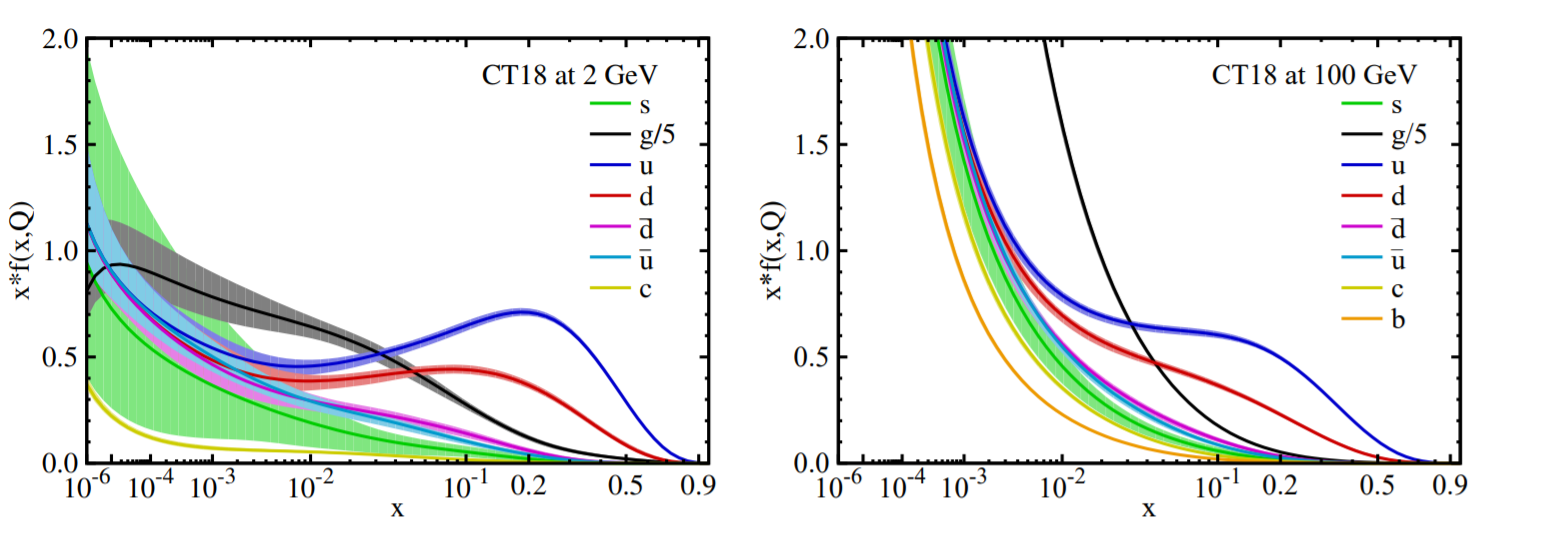
\includegraphics[width=\linewidth]{CT18_PDF.png}
	\caption{\label{fig:PDFs}
		CTEQ-TEA kolektyvo pateikiamos protono partonų pasiskirstymo funkcijos esant skirtingoms susidūrimų energijoms \cite{CTEQ2019}.
		Kairėje -- $Q=2 \; \mathrm{GeV}$, dešinėje -- $Q=100 \; \mathrm{GeV}$.
		Ant horizontalios ašies vaizduojama protono impulso dalis $x$, o ant vertikalios -- tikimybės tankio $f(x,\, Q^2)$
		ir $x$ sandauga.}
\end{figure}

\subsubsection{Drell-Yan procesas}

Drell-Yan procesas \cite{DYoriginal} -- tai toks procesas, kai protonų susidūrimo metu anihiliavus kvarkui ir antikvarkui
sukuriama leptono ir antileptono pora.
Šis procesas vyksta apsikeičiant $Z$ bozonu arba virtualiu fotonu per s-kanalą (\ref{fig:DYfeyn}):

\begin{equation*}
	q\bar{q} \rightarrow Z/ \gamma^{*} \rightarrow l^{+}l^{-} \; .
\end{equation*}
Toliau bus žymima $\DY \! \rightarrow \! l^{+}l^{-}$.
Skirtingos Drell-Yan proceso galutinės būsenos, priklausomai nuo to, kokios rūšies leptonai susidaro, yra
vadinamos kanalais: elektronų kanalas, miuonų kanalas, taonų kanalas.
Kadangi taonai gyvuoja labai trumpai, jų kanalo tyrimas yra sudėtingesnis ir dažniausiai yra vykdomas atskirai,
o tuo tarpu elektronų ir miuonų kanalo tyrimus neretai vykdo ta pati mokslinė grupė.

Drell-Yan procesas tapo svarbiu tyrimo objektu nuo pat pirmojo jo aprašymo $1970$-aisiais
metais, kai S.\ D.\ Drell ir T.\ M.\ Yan bandė apibūdinti leptonų ir antileptonų porų susidarymą
hadronų susidūrimų metu \cite{DYoriginal}.
Drell-Yan procesas pirmą kartą eksperimentiškai buvo stebėtas dar tais pačiais metais protonų susidūrimuose
su urano branduoliais \cite{DY_firstExp}.
Šio proceso tyrimas svarbus todėl, kad jame dalyvauja nevaletintis protono kvarkas.
Tai leidžia padaryti svarbių įžvalgų apie protono sandarą.

Šiais laikais Drell-Yan procesas teoretikų gali būti sėkmingai aprašomas iki trečios eilės kvantinės chromodinamikos
perturbacijų tikslumo (angl.\ \textit{next-to-next-to-leading order} -- NNLO reiškia dviejų kilpų ir dviejų
dalelių išspinduliavimo pataisas).
Tokios aukštos eilės elektrosilpnosios pataisos nenaudojamos, nes kiekvienos elektrosilpnosios viršūnės
indėlis į reakcijos skerspjūvį yra $>10$ kartų mažiau reikšmingas, lyginant su stipriosios sąveikos viršūne.
Didelio tikslumo eksperimentiniai Drell-Yan proceso diferencialinio skerspjūvio matavimai \cite{DY2013, DY7TeVatlas, DY2015, DY8TeVatlas, DY2019}
naudojami ne tik partonų pasiskirstymo funkcijoms tikslinti, bet taip pat ir perturbacinės kvantinės
chromodinamikos bei elektrosilpnosios sąveikos teorijoms tikrinti.
Be to, šis procesas yra vienu iš pagrindinių triukšmo procesų įvairiuose kituose didelių energijų fizikos tyrimuose,
pavyzdžiui, Higso bozono tyrime \cite{Higgs2018}, ne standartinio modelio dalelės -- $Z'$ bozono -- paieškoje \cite{Zprime},
supersimetrijos paieškoje \cite{SUSYtau} ir pan.
Taigi, tikslūs Drell-Yan proceso matavimai įvairiapusiškai prisideda prie kitų didelių energijų
fizikos tyrimų rezultatų kokybės.

\begin{figure}[H]
\centering
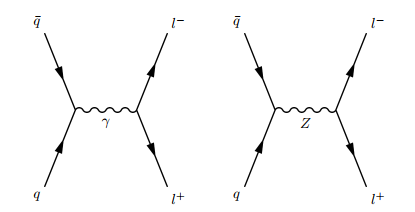
\includegraphics[scale=0.75]{DYprocess.PNG}
\caption{Drell-Yan procesą apibūdinančios medžio lygmens Feinmano diagramos.}
\label{fig:DYfeyn}
\end{figure}

\subsubsection{Čiurkšlės}

Vykdant protonų susidūrimus galutinė įvykio būsena dažnai yra palydima vieno ar kelių kvarkų ir/arba gliuonų
(neskaitant likusių partonų, kurie protonams susiduriant tarpusavyje nesureaguoja ir nulekia apytiksliai tiesiai).
Pavyzdžiui, energingą kvarką arba gliuoną prieš sąveikaudami gali išspinduliuoti reakcijoje dalyvaujantys partonai,
taip pat įvykio metu sukurtos masyvios dalelės (tokios, kaip taonai, $W$, $Z$ ir Higso bozonai) su tam tikra
tikimybe gali skilti į kvarkus ir pan.
Vis dėlto, pavieniai kvarkai arba gliuonai dalelių detektoriais niekada nebūna aptinkami.
Energingi kvarkai arba gliuonai nuolat praranda energiją spinduliuodami papildomus gliuonus, o gliuonai savo ruožtu
dar gali skilti į kvarko-antikvarko poras.
Tokiu būdu lėkdamas vienas partonas sukuria taip vadinamą \ltq{partonų dušą} (angl. \textit{parton shower}).
Galiausiai partonų duše esančių dalelių energija pasidaro pakankamai maža, kad perturbatyvusis kvantinės chromodinamikos
aprašymas joms nebetinka -- sąveikos konstanta yra labai didelė, kvarkus atskirti vieną nuo kito reikia begalinės energijos.
Žemose energijose ($<1$ GeV) pasireiškia kvarkų \ltq{įkalinimas} (angl. \textit{confinement}): dėl sąveikos stiprumo
kvarkai gali egzistuoti tik grupėmis, kuriose spalvinis krūvis neutralizuojamas.
Taigi, partonų duše esantys kvarkai ir gliuonai pradeda formuoti hadronus (šis procesas vadinamas hadronizacija)
ir vieno energingo partono pėdsaką detektoriuje užfiksuojame kaip kūgio formos dalelių srautą, sudarytą iš daugybės
įvairių rūšių hadronų \cite{Jets}.
Šie hadronų srautai vadinami čiurkšlėmis (angl. \textit{jets}).

Vis dėlto, nebūtinai visos čiurkšlėse susidarančios dalelės yra hadronai.
Hadronizacijos proceso metu neretai gali susiformuoti ir fotonai (pavyzdžiui, neutralaus piono skilimo metu).
Taip pat protonų susidūrimo metu vykstant didelės energijos partonų sklaidos procesams galima sukurti sunkiųjų kvarkų,
kurie skyla leptoniškai.
Pavyzdžiui, elektronas arba miuonas gali būti randamas apytiksliai $20\%$ gelminio kvarko sukurtų čiurkšlių
(angl. \textit{b-jets}) ir apytiksliai $10\%$ žaviojo kvarko sukurtų čiurkšlių (angl. \textit{c-jets}) \cite{LeptonJets}.
Čiurkšlėse susidariusios stipriąja sąveika nesąveikaujančios dalelės neretai pagelbėja mokslininkams nustatant,
kokį kvarką atitinka matoma čiurkšlė \cite{LeptonJets}, tačiau taip pat gali ir suklaidinti -- kartais čiurkšlė gali
būti supainiojama su protonų susidūrimo metu pagamintu leptonu \cite{DY2013, DY7TeVatlas, DY2015, DY8TeVatlas, DY2019, EleID, MuonID}.

\subsection{Eksperimentinis Drell-Yan proceso tyrimas}

\subsubsection{Didysis hadronų greitintuvas ir Kompaktiškasis miuonų solenoidas}

Europos branduolinių tyrimų organizacijai CERN priklausantis Didysis hadronų greitintuvas
(angl.\ \textit{Large Hadron Collider} -- LHC) yra didžiausias ir galingiausias dalelių greitintuvas pasaulyje.
Tai yra $~100$ m gylyje po žeme esantis žiedinis greitintuvas, kurio perimetras siekia $27$ km \cite{LHC}.
Nuo $2015$ metų Didžiajame hadronų greitintuve vykdomi $13$ TeV energijos protonų susidūrimai.
Beveik visi susidūrimai vyksta kas $25$ ns keliuose skirtinguose žiedo taškuose, aplink kuriuos yra išdėstyti dalelių
detektoriai, priklausantys skirtingų eksperimentų grupėms.

Kompaktiškasis miuonų solenoidas (angl.\ \textit{Compact Muon Solenoid} -- CMS) \cite{CMSexperiment}
yra plačios paskirties
detektorius, galintis detektuoti skirtingas daleles.
CMS yra cilindrinės geometrijos, jo aukštis ir plotis -- apytiksliai po $15$ m, o ilgis --
apie $21$ m.
Detektoriaus masė siekia apie $14000$ tonų, jis susideda iš daug sluoksnių ir segmentų, kurie skirti
detektuoti skirtingų rūšių dalelėms.
Svarbiausia CMS dalis -- didžiausias pasaulyje solenoidinis elektromagnetas.
Tai -- iki superlaidumo temperatūros atšaldoma ritė, kuria darbo metu teka maždaug $19.1$ kA stiprio
elektros srovė, ir kurios viduje sukuriamas iki $4$ T siekiantis magnetinis laukas.

\vspace{0.2cm}
\begin{figure}[H]
	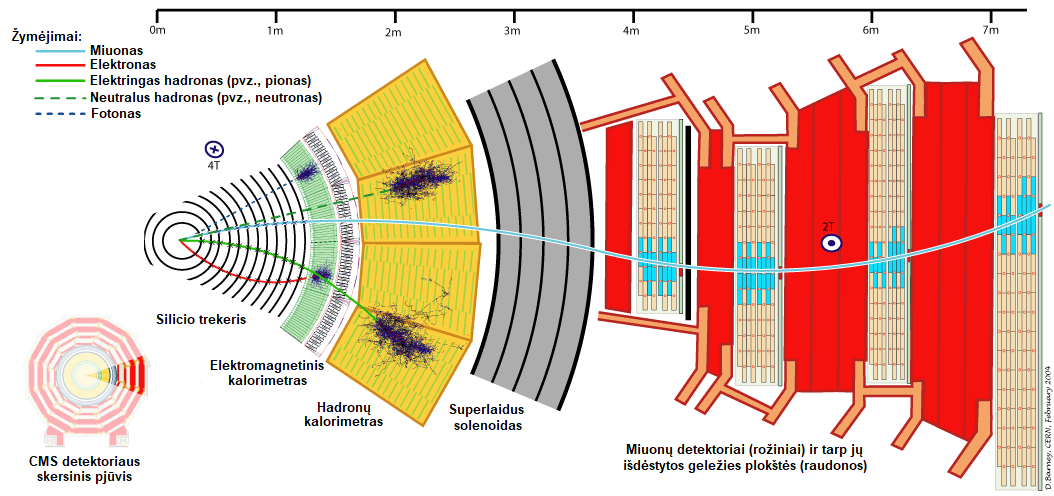
\includegraphics[width=\textwidth]{CMSslice_LT.png}
	\caption{\label{fig:CMSslice}Skersinis CMS detektoriaus pjūvis \cite{CMSslice}.
	Skirtingos linijos žymi įvairių dalelių, išlekiančių iš protonų susidūrimo vietos, trajektorijas.
	Trūki linija žymi elektriškai neutralios dalelės trajektoriją, kuri silicio trekų detektoriuje
	neužfiksuojama.}
\end{figure}

CMS detektoriaus sluoksnius galima pamatyti \ref{fig:CMSslice} paveiksle.
Kiekvienas subdetektorius turi vieną cilindrinę ir dvi antgalių dalis, kurios yra išdėstytos sluoksniais
aplink protonų susidūrimo vietą.
Subdetektorių sluoksniai yra išdėstyti atsižvelgiant į detektuojamų dalelių skvarbą, kiekvienas sluosknis
yra skirtingas ir turi savo paskirtį \cite{CMSexperiment}.

Išsaugoti kiekvieną kas $25$ ns vykstantį įvykį fiziškai yra labai sudėtinga: vienas įvykis užima apie
$1$ MB \cite{CMScomputing}, taigi reikėtų ypatingai greitos elektronikos, galinčios išrašyti $~40$ TB duomenų
per sekundę.
Taip pat reikėtų didžiulių duomenų saugojimo pajėgumų, o tai nėra optimalu turint omenyje, jog labai didelė dalis
visų įvykių tyrėjams nebus įdomus (nepakankamai didelės energijos reakcijos, jau pakankamai ištirti procesai ir pan.).
Taigi, išsaugomų įvykių skaičiui sumažinti naudojama dviejų lygių trigerių sistema \cite{CMStrig}.
Pirmojo lygio trigeris -- tai šalia detektoriaus sumontuota specialiai tam sukurta kompiuterinės
įrangos sistema.
Joje realiu laiku minimaliai apdorojami kalorimetrų bei miuonų detektorių duomenys ir pagal juos per
$4 \; \mathrm{\mu s}$ sistema nusprendžia, ar įvykis turėtų būti išsaugomas tolimesnei analizei. 
Pirmojo lygio trigeris išsaugo maždaug $1$ įvykį iš $10000$.
Aukšto lygio trigeris -- tai superkompiuterių sistema, į kurią atkeliauja pirmojo lygio trigerį
aktyvavę įvykiai.
Čia įvykiai atkuriami pasinaudojant pilna detektoriaus užregistruota informacija, naudojami
griežtesni atrankos kriterijai.
Tai padeda įvykių skaičių sumažinti iki maždaug $1000$ įvykių per sekundę.
Pastarieji yra įrašomi ilgalaikiam saugojimui, kad vėliau galėtų būti analizuojami mokslininkų.

Protonų susidūrimo įvykio vaizdas, pasinaudojant detektoriaus užregistruota informacija, atkuriamas naudojantis
dalelių srauto (angl. \textit{Particle Flow}) algoritmu \cite{ParticleFlow}.
Šis algoritmas bando susieti trekų detektoriuje užregistruotus signalus su pataikymais į kalorimetrus arba miuonų
detektorius, taip nustatydamas, kokios dalelės susidarė ir kokie jų parametrai (krūvis, skersinis impulsas,
skersinė energija, pseudosparta ir pan.).
Tokiu būdu gaunamas platus galutinių įvykio produktų sąrašas, leidžiantis pamatyti pilną protonų susidūrimo įvykio vaizdą,
kurį jau gali analizuoti mokslinės tyrimų grupės.

\subsubsection{Signalas ir triukšmas}

Drell-Yan proceso metu susidaro du priešingo elektrinio krūvio izoliuoti (neturintys šalia esančių pašalinių dalelių trajektorijų) leptonai.
Detektoriuje panašiai atrodanti leptonų pora gali susidaryti ir kitų procesų metu.
Taip pat pasitaiko atvejų, kai čiurkšlės arba jose susidarę leptonai yra klaidingai atpažįstami kaip izoliuoti leptonai.
Visi įvykiai, kurie analizuojant duomenis atrodo kaip Drell-Yan (signalo) procesas, tačiau tokie nėra, vadinami
\ltq{triukšmo įvykiais}.
Pagrindiniai Drell-Yan proceso triukšmai yra šie: viršūninių kvarkų poros ($t\bar{t}\,$) įvykiai, dviejų masyvių vektorinių bozonų
įvykiai ($WW$, $WZ$ ir $ZZ$), vieno viršūninio kvarko ir $W$ bozono įvykiai ($tW$ arba $\bar{t}W$), $W$ bozono
ir čiurkšlės įvykiai ($\WJets$) bei stipriosios sąveikos nulemti kelių čiurkšlių įvykiai (sutrumpintai vadinami $\QCD$).
Taip pat tiriant Drell-Yan proceso elektronų ir miuonų kanalus vienas iš svarbių triukšmų yra
to paties Drell-Yan proceso taonų kanalas $\DYtau$, kai taonai skyla į elektronus arba miuonus.
Stengiantis išskirti, kokią dalį detektoriaus registruojamuose pasiskirstymuose sudaro signalo (Drell-Yan),
o kokią -- triukšmo įvykiai, gali būti pasitelkiamas Monte Carlo (MC) modeliavimas ir/arba matavimu grįsti metodai.

\textbf{Monte Carlo modeliavimas} -- tai Monte Carlo metodu sumodeliuoti protonų susidūrimo įvykiai.
Įvykių modeliavimas atliekamas keliais lygmenimis.
Pirmiausia sumodeliuojamas pats protonų susidūrimas ir gaunama, kokios dalelės susidarė jo metu.
Tada modeliuojami po susidūrimo vykstantys antriniai procesai, tokie, kaip hadronizacija, spinduliavimas, dalelių skilimai,
pašaliniai mažos energijos protonų susidūrimai, vykstantys tuo pačiu metu (angl. \textit{pile-up}).
Galiausiai modeliuojama, kaip įvykio produktai sąveikauja su medžiaga -- detektoriaus komponentais.
Tokį virtualų eksperimentą kartojant daug kartų galima gauti vidutinį rezultatą, kuris yra palyginamas su realiu eksperimentu.
Vis dėlto, sumodeliuoti įvykius taip, kad virtualaus eksperimento sąlygos idealiai atitiktų realaus eksperimento sąlygas,
yra praktiškai neįmanoma.
Norint atsižvelgti į kai kuriuos iš neatitikimų modeliuotiems įvykiams gali būti pritaikomos CMS eksperimento mokslinių grupių
rekomenduojamos pataisos.
Tačiau vis tiek egzistuoja neapibrėžtumų, tokių, kaip nepakankamos žinios apie atskirų triukšmo procesų įvykių tikėtinumus,
neidealus detektoriaus atsako modeliavimas, papildomi protonų susidūrimai ir pan., kurie kenkia įverčio kokybei.
Šių problemų gali būti išvengiama triukšmo įvykių skaičiaus įvertinimui naudojant matavimu grįstus metodus.

\textbf{Matavimu grįsti metodai} apjungia matavimą ir modeliavimą, kad būtų gautas kuo tikroviškesnis įvykių skaičiaus įvertis.
Matavimu grįstų metodų veikimo principas remiasi signalo ir kontrolinės sričių apibrėžimais.
Signalo sritis -- tai sritis, pasirinkta taip, kad į ją patektų kuo daugiau signalo ir kuo mažiau triukšmo įvykių.
Kontrolinė sritis -- tai taip pasirinkta sritis, kad į ją patektų kuo daugiau triukšmo ir kuo mažiau signalo įvykių.
Sritys apibrėžiamos tam tikrais užregistruotus įvykius apibūdinančių parametrų apribojimais.
Šie parametrai gali būti įvairūs: tam tikrų dalelių ar čiurkšlių skaičius, trajektorijų izoliuotumas ir pan.
Signalo ir kontrolinė sritys turi būti nepersiklojančios.
Skirtingi matavimu grįsti metodai skirtingais būdais transformuoja triukšmo įvykių skaičių, apskaičiuotą kontrolinėje
srityje, į triukšmo įvykių skaičių, esantį signalo srityje.
$\emu$ metodas naudojamas įvertinti indėliui triukšmų, siejamų su procesais, kurių metu susidariusios dvi nestabilios dalelės
skyla į leptonus nepriklausomai.
Taip pat eksperimentinėje didelių energijų fizikoje ganėtinai populiarūs yra klaidingo fizikinio objekto atpažinimo ir ABCD metodai.
Jie naudojami įvertinti skaičiui tokių triukšmo įvykių, kurių metu susidaro viena ar kelios čiurkšlės.

\paragraph{$\emu$ metodas\\}

$\emu$ metodas yra tinkamas įvertinti triukšmo įvykių skaičiui tokių procesų, kurių metu susidaro dvi
nestabilios dalelės, galinčios nepriklausomai skilti į vienodų arba skirtingų rūšių leptonus.
Tokio proceso pavyzdžiai yra $WW$, $tW$, $\tbarW$, $\ttbar$ ir $\DYtau$.
$WW$ proceso atveju, nagrinėjant tik leptoninius skilimus, atmetant skilimą į taonus bei nekreipiant dėmesio į skilimo metu
susidarančius neutrinus, galimos tokios įvykio baigtys: $WW\rightarrow e^{+} e^{-}$, $WW\rightarrow e^{+}\mu^{-}$,
$WW\rightarrow \mu^{+}e^{-}$, $WW\rightarrow \mu^{+}\mu^{-}$.
Taikant $\emu$ metodą signalo sritis -- $ee$ arba $\mu\mu$ įvykiai.
Tuo tarpu kontrolinė sritis -- įvykiai, kuriuose susidarė vienas elektronas ir vienas miuonas ($\emu$ įvykiai).
Tokios būsenos neįmanoma gauti iš Drell-Yan proceso signalo, taigi joje bus vien triukšmo įvykiai.
Triukšmo įvykių skaičius iš kontrolinės srities ($\emu$) į signalo sritį ($ee$ arba $\mu\mu$)
transformuojamas pasinaudojant Monte Carlo modeliavimo rezultatais:

\begin{equation}
	N_{\mu\mu}^{\mathrm{Tr. \, įvert.}} =
	\frac{ N_{\mu\mu}^{\mathrm{Tr. \, MC}} }{ N_{e\mu}^{\mathrm{Tr. \, MC}} }
	\cdot N_{e\mu}^{\mathrm{Tr. \, eksp.}} \; ,
	\label{eq:emuMethod}
\end{equation}
čia $N_{\mu\mu}^{\mathrm{Tr. \, įvert.}}$ -- $\emu$ metodu įvertintas triukšmo įvykių skaičius signalo srityje,
$N_{e\mu}^{\mathrm{Tr. \, eksp.}}$ -- į kontrolinę sritį patenkančių detektoriumi užregistruotų įvykių skaičius,
$N_{\mu\mu}^{\mathrm{Tr. \, MC}}$ ir $N_{e\mu}^{\mathrm{Tr. \, MC}}$ -- modeliuotų triukšmo įvykių skaičius
atitinkamai signalo ir kontrolinėje srityje.
$\emu$ metodo įvertis buvo gautas ankstesniame darbe, o šiame darbe gilinamasi į klaidingo atpažinimo metodą.

\paragraph{Klaidingo atpažinimo metodas\\}

Klaidingo fizikinio objekto atpažinimo (angl. \textit{fake rate}) metodas yra naudojamas įvertinti skaičiui triukšmo įvykių,
kurie užregistruojami įvykio atkūrimo algoritmui neteisingai atpažinus vieną ar kelis fizikinius objektus.
Pavyzdžiui, fotonas gali būti klaidingai atpažintas kaip elektronas, čiurkšlė klaidingai atpažinta kaip elektronas
arba miuonas ir pan.
Klaidingo atpažinimo metodas remiasi tikimybės, kad klaidingai atpažintas fizikinis objektas pateks į signalo sritį
(angliškai ši tikimybė vadinama \textit{fake rate}), įvertinimu ir pritaikymu triukšmo įvykių skaičiui, įvertintam
kontrolinėje srityje, transformuoti į triukšmo įvykių skaičių, patenkantį į signalo sritį.

Klaidingo atpažinimo metodo atveju kontrolinė sritis įprastai apibrėžiama invertuojant tam tikrą įvykių atrankos kriterijų, naudojamą
atskirti teisingai atpažintam fizikiniam objektui nuo atpažinto blogai.
Norint nustatyti tikimybę, kad čiurkšlė bus klaidingai atpažinta kaip miuonas, dažniausiai invertuojamas trajektorijos izoliuotumo
reikalavimas -- reikalaujama, kad miuono kandidato trajektorija būtų neizoliuota nuo kitų dalelių trajektorijų, o tai neretai yra
čiurkšlės arba miuono, susidariusio čiurkšlėje, požymis.
Tada klaidingo atpažinimo tikimybe vadiname dydį, nusakantį, kokia dalis visų kaip miuonai atpažintų čiurkšlių turi galimybę patekti
į signalo sritį:
\begin{equation} \label{eq:FR}
	f_{\mathrm{signal} \,| \,\mathrm{Jet}} =
	\frac{N^{\QCD}_{\mathrm{signal}}}{N^{\QCD}_{\mathrm{signal}}+N^{\QCD}_{\mathrm{control}}} \; ,
\end{equation}
čia $f_{\mathrm{signal} \,| \,\mathrm{Jet}}$ -- klaidingo atpažinimo tikimybė, $N^{\QCD}_{\mathrm{signal}}$ -- į signalo sritį
patenkančių kaip miuonai atpažintų čiurkšlių skaičius, $N^{\QCD}_{\mathrm{control}}$ -- į kontrolinę sritį patenkančių kaip miuonai
atpažintų čiurkšlių skaičius.
Indeksas $\QCD$ žymi faktą, kad klaidingo atpažinimo tikimybės įvertinimui turėtume naudoti tik $\QCD$ įvykius, t.y., įvykius,
kuriuose susidaro vien tik čiurkšlės, todėl bet koks tokiuose įvykiuose atpažintas miuonas yra kilęs iš čiurkšlės.

Apskaičiavus klaidingo atpažinimo tikimybę galima ją pritaikyti įvertinant, koks kiekis klaidingai atpažintų fizikinių objektų
galėjo patekti į signalo sritį.
Drell-Yan proceso atveju, kai ieškoma dviejų leptonų, galimas dvejopas klaidingo atpažinimo nulemtas triukšmas: klaidingai gali būti
atpažintas tik vienas leptonas, arba abu.
Pilnas į signalo sritį patenkančių įvykių skaičius gali būti išreikštas taip:
\begin{multline}
	\label{eq:realfake}
	N_{\mathrm{signal, \; signal}} = N_{l, \, l} \cdot f_{\mathrm{signal} \,| \,l} \cdot f_{\mathrm{signal} \,| \, l} +
	N_{l, \, \mathrm{Jet}} \cdot f_{\mathrm{signal} \,| \, l} \cdot f_{\mathrm{signal} \,| \,\mathrm{Jet}} + \\[5pt] +
	N_{\mathrm{Jet, \, Jet}} \cdot f_{\mathrm{signal} \,| \,\mathrm{Jet}} \cdot f_{\mathrm{signal} \,| \,\mathrm{Jet}} \, ,
\end{multline}
čia $l$ žymi tikrą leptoną, $N_{l, \, l}$, $N_{l, \, \mathrm{Jet}}$, $N_{\mathrm{Jet, \, Jet}}$ -- įvykių,
kurių metu susidarė atitinkamai du leptonai, leptonas ir čiurkšlė, arba dvi čiurkšlės, skaičius,
$f_{\mathrm{signal} \,| \,\mathrm{Jet}}$ -- klaidingo atpažinimo tikimybė, $f_{\mathrm{signal} \,| \,l}$ -- tikimybė,
kad tikras leptonas bus atpažintas teisingai (dar vadinama efektyvumu).
\eqref{eq:realfake} lygybės dešinė pusė susideda iš trijų dėmenų.
Pirmasis dėmuo yra siejamas su tikrų leptonų įvykiais: Drell-Yan signalu ir triukšmo procesais, kurių metu susidaro tikri leptonai.
Antrasis dėmuo yra siejamas su vieno tikro leptono ir vienos klaidingai apažintos čiurkšlės įvykiais
(dominuojantis procesas -- $\WJets$), o trečiasis -- su dviejų klaidingai apažintų čiurkšlių įvykiais -- $\QCD$ triukšmu.
Pritaikę klaidingo atpažinimo tikimybę galime įvertinti \eqref{eq:realfake} išraiškos dešinėje pusėje esančius antrąjį ir trečiąjį dėmenis.
Antrajame dėmenyje esantis $N_{l, \, \mathrm{Jet}}$ gali būti įvertintas pasinaudojus įvykiais, kuriuose susidarė vienas tikras
leptonas, patenkantis į signalo sritį, ir viena klaidingai atpažinta čiurkšlė, patenkanti į kontrolinę sritį:
\begin{equation}
	\label{eq:FRWjets}
	N_{l, \, \mathrm{Jet}} = \frac{N^{\WJets}_{\mathrm{signal, \, control}}}
	{f_{\mathrm{signal} \,| \, l}\cdot f_{\mathrm{control} \,| \, \mathrm{Jet}}} =
	\frac{N^{\WJets}_{\mathrm{signal, \, control}}}
	{f_{\mathrm{signal} \,| \, l}\cdot \left( 1 - f_{\mathrm{signal} \,| \, \mathrm{Jet}} \right)}	\, ,
\end{equation}
čia $N^{\WJets}_{\mathrm{signal, \, control}}$ -- $\WJets$ įvykių skaičius, kurių metu susidariusi čiurkšlė
klaidingai atpažįstama, bet patenka į kontrolinę sritį.
Trečiajame \eqref{eq:realfake} išraiškos dėmenyje esantis $N_{\mathrm{Jet, \, Jet}}$ gali būti įvertintas pasinaudojus įvykiais,
kuriuose dvi klaidingai atpažintos čiurkšlės patenka į kontrolinę sritį:
\begin{equation}
	\label{eq:FRQCD}
	N_{\mathrm{Jet, \, Jet}} = \frac{N^{\QCD}_{\mathrm{control, \, control}}}{f_{\mathrm{control} \,| \,\mathrm{Jet}} \cdot
	f_{\mathrm{control} \,| \,\mathrm{Jet}}} = \frac{N^{\QCD}_{\mathrm{control, \, control}}}
	{\left(1-f_{\mathrm{signal} \,| \,\mathrm{Jet}}\right) \cdot \left(1-f_{\mathrm{signal} \,| \,\mathrm{Jet}}\right)} \, ,
\end{equation}
čia $N^{\QCD}_{\mathrm{control, \, control}}$ -- $\QCD$ įvykių skaičius, kuriuose dvi klaidingai atpažintos čiurkšlės patenka į
kontrolinę sritį.
Įstatę \eqref{eq:FRWjets} ir \eqref{eq:FRQCD} išraiškas į \eqref{eq:realfake}, gauname:
\begin{multline}
	\label{eq:FRapply}
	N_{\mathrm{signal, \; signal}} = N_{l, \, l} \cdot f_{\mathrm{signal} \,| \,l} \cdot f_{\mathrm{signal} \,| \, l} +
	N^{\WJets}_{\mathrm{signal, \, control}} \cdot
	\frac{f_{\mathrm{signal} \,| \, \mathrm{Jet}}} {1 - f_{\mathrm{signal} \,| \, \mathrm{Jet}}} + \\[5pt] +
	N^{\QCD}_{\mathrm{control, \, control}} \cdot
	\frac{f_{\mathrm{signal} \,| \,\mathrm{Jet}} \cdot f_{\mathrm{signal} \,| \,\mathrm{Jet}}}
	{\left(1-f_{\mathrm{signal} \,| \,\mathrm{Jet}} \right) \cdot \left(1-f_{\mathrm{signal} \,| \,\mathrm{Jet}} \right)}\, .
\end{multline}
Taigi, įvertinus klaidingo atpažinimo tikimybę $f_{\mathrm{signal} \,| \,\mathrm{Jet}}$, $QCD$ ir $\WJets$ triukšmo įvykių
skaičių galima įvertinti apskaičiuojant šių įvykių skaičių kontrolinėje srityje ir perkeliant gautą rezultatą į
signalo sritį pasinaudojus reikiamu skaičiumi daugiklių
$f_{\mathrm{signal} \,| \,\mathrm{Jet}}/(1-f_{\mathrm{signal} \,| \,\mathrm{Jet}})$.

\section{Drell-Yan proceso tyrimo metodika}

Šiame skyriuje pateikiama pagrindinė informacija apie tai, kaip buvo atliekamas tyrimas: pristatomi naudoti
duomenų rinkiniai, trumpai apibūdinami įvykių atrankos kriterijai, nurodomos pritaikytos pataisos, detaliau apibūdinamas
Drell-Yan proceso triukšmo įvykių skaičiaus įvertinimui naudotas klaidingo fizikinio objekto atpažinimo metodas,
pristatomi taikyti paklaidų įvertinimo principai.
Ankstesniame skyriuje išsakytos idėjos yra tinkamos tiek $\DYee$, tiek $\DYmumu$ procesų tyrimams, tačiau šiame skyriuje
koncentruojamasi į Drell-Yan proceso miuonų kanalą, nes pristatomas darbas buvo atliktas būtent šiame kanale.

\subsection{Duomenų rinkiniai ir analizės kodai}

Šiame darbe buvo naudojami dalinai apdoroti CERN CMS detektoriaus 2016 metais užregistruoti $13$ TeV
energijos protonų susidūrimų duomenys.
Duomenų kiekis atitinka $35.9$ \invfb integruotąjį šviesį, arba $~2 \cdot 10^{15}$ protonų susidūrimų.
Tai yra $>10$ kartų daugiau įvykių, nei užregistruota $2015$-aisiais metais \cite{DY2019}.

Detektoriaus duomenų interpretavimui bei matavimu grįstam triukšmo įvykių skaičiaus įvertinimui
buvo pasitelkiami modeliuoto Drell-Yan signalo bei pagrindinių triukšmo procesų duomenų rinkiniai.
Drell-Yan signalo bei $\WJets$ proceso įvykiai buvo sumodeliuoti antros eilės kvantinės chromodinamikos
perturbacijų tikslumu  (angl. \textit{next-to-leading order} -- NLO) naudojant \textsc{MadGraph5\_aMC@NLO} įvykių
modeliavimo programą \cite{MG_aMCatNLO}.
Viršūninio-antiviršūninio kvarko poros ($t\bar{t}\,$) ir vieno viršūninio kvarko kartu su $W$ bozonu ($tW$ arba
$\bar{t}W$) įvykiai buvo sumodeliuoti naudojant \textsc{Powheg} \cite{powheg_ttbar, powheg_tW}.
\textsc{Powheg} taip pat įvykius modeliuoja antros eilės QCD perturbacijų tikslumu.
Dviejų bozonų ($WW$, $WZ$, $ZZ$) įvykiai buvo sumodeliuoti su \textsc{Pythia8} nulinės eilės perturbacijų tikslumu
(angl. \textit{leading order} -- LO) \cite{pythia82}.
Visų modeliuotų įvykių metu vykstantys antriniai procesai, tokie, kaip hadronizacija, spinduliavimas, dalelių skilimai,
pašaliniai protonų susidūrimai ir pan., buvo sumodeliuoti naudojantis \textsc{Pythia8}.
Detektoriaus atsakas į kiekvieną iš sumodeliuotų įvykių buvo modeliuojamas naudojantis \textsc{Geant4} programa
\cite{geant4}.

Darbe naudoti CMS Drell-Yan tyrimo grupės dalinai atrinkti duomenys saugomi Pietų Korėjoje esančiame CMS Tier2
duomenų centre ir užima apie $14$ TB.
Duomenų analizei buvo rašomi C++ programiniai moduliai, kurie buvo leidžiami ROOT aplinkoje \cite{ROOTarticle}.
Duomenų analizė vykdyta dviem etapais: pirmiausia buvo atliekama išmatuotų ir modeliuotų įvykių atranka nuotoliniu
būdu prisijungus prie skaičiavimo centro.
Svarbiausia su atrinktais įvykiais susijusi informacija buvo įrašoma į naujus duomenų failus, kurie užima tik
apie $10$ GB.
Naujai sukurti failai buvo parsisiunčiami į vietinį kompiuterį tolimesnei analizei.
Programinio kodo versijos buvo tvarkomos naudojantis \textit{Github} versijų valdymo sistema.
Visi parašyti analizės kodai yra patalpinti \textit{Github} saugykloje, esančioje adresu
\url{https://github.com/marijusambrozas/DrellYan2016/tree/master/SelectedX}.

\subsection{Įvykių atranka}\label{sec:selection}
Norint iš $2016$-aisiais metais CMS detektoriaus užregistruotų duomenų išskirti svarbią ir kokybišką informaciją
buvo vykdoma įvykių atranka pagal kriterijus, kurie turėtų atmesti kiek įmanoma daugiau triukšmo įvykių ir tuo pačiu
išsaugoti kuo daugiau signalo įvykių.
Taip pat buvo apribojama tyrimo fazinė erdvė, paliekant tik tas sritis, kuriose detektoriaus veikimas yra efektyviausias.
Visi taikyti atrankos kriterijai yra pateikti \ref{table:selection} lentelėje.

Pirmiausia atrenkant įvykiųs buvo naudojamas aukšto lygio vieno miuono trigeris, kuris aktyvuojamas aptikus bent vieną
miuoną su skersiniu impulsu, didesniu nei $24$ GeV.
Miuonas turi būti atpažintas pasinaudojant trekų detektoriaus ir miuonų detektorių informacija.
Kiekvienam miuonui iš trigerį aktyvavusių įvykių buvo taikomi \ttt{TightID} reikalavimai \cite{MuonID}, skirti sumažinti atranką
praeinančių netikrų miuonų, bei miuonų, atsiradusių iš antrinių procesų, skaičių.
\ttt{TightID} reikalavimus atitinka virš $95\%$ protonų susidūrimų metu sukurtų tikrų ir mažiau nei $0.3\%$ netikrų
miuonų \cite{MuonID}.
Taip pat kiekvienam miuonui buvo taikomas trajektorijos izoliuotumo reikalavimas: pašalinių dalelių, aptiktų
$\Delta R = \sqrt{(\Delta\eta)^2 + (\Delta\phi)^2} < 0.3$ (čia $\eta$ -- pseudosparta, $\phi$ -- azimutinis kampas)
pločio kūgyje, nubrėžtame aplink miuono trajektoriją, skersinių impulsų suma negali
viršyti $15\%$ miuono skersinio impulso vertės: $I_{\mathrm{PF}}^{\mathrm{rel.}}<0.15$ (čia \ltq{PF} žymi tai, jog
šį dydį apskaičiuoja dalelių srauto algoritmas).
Įvykiai, kuriuose nėra bent dviejų miuonų, atitinkančių išvardintus kriterijus buvo iškart atmetami.
Likusiems įvykiams buvo taikomas reikalavimas, kad miuonų poros trajektorijas pakankamai tiksliai eitų suvesti į vieną pirminę
viršūnę, taip pat buvo reikalaujama bei kad suporuoti miuonai būtų priešingų elektrinių krūvių.
Įvykyje esant kelioms reikalavimus atitinkančioms poroms iš jų buvo išrenkama ta, kurią eina tiksliausiai suvesti į bendrą viršūnę
Tam, kad būtų išvengta kosminės spinduliuotės miuonų aptikimo, buvo taikomas papildomas kriterijus, reikalaujantis,
kad plokštuminis kampas tarp dviejų miuonų trajektorijų būtų mažesnis, nei $\pi-0.005$ rad.

Pagrindinis matuojamas dydis buvo atranką praėjusių miuonų porų invariantinė masė.
Iš jų verčių buvo brėžiama invariantinės masės histograma, apimanti masės sritį nuo $15$ iki $3000$ GeV.

\begin{table}
	\begin{tabular}{|c|c|}
		\hline
		\textbf{Kriterijaus tipas} & \textbf{Reikalavimas} \\
		\hline\hline
		\multirow{3}{12em}{\centering Trigeris} & \ttt{HLT\_IsoMu24} arba \ttt{HLT\_IsoTkMu24} \\ \cline{2-2}
			& \multirow{2}{17em}{\centering Bent vienas miuonas turi būti aktyvavęs trigerį} \\
		 & \\
		\hline\hline
		\multirow{2}{12em}{\centering Kinematiniai reikalavimai} & $p_{\mathrm{T \, 1}} > 28$ GeV, $p_{\mathrm{T \, 2}} > 17$ GeV \\ \cline{2-2}
		 & $|\eta_1| < 2.4$, $|\eta_2| < 2.4$ \\
		\hline\hline
		\multirow{2}{12em}{\centering Dalelės identifikavimo reikalavimai} & \ttt{TightID} reikalavimai \\ \cline{2-2}
		 & $I_{\mathrm{PF}}^{\mathrm{rel.}}<0.15$ \\
		\hline\hline
		\multirow{5}{12em}{\centering Reikalavimai geresniam signalo išskyrimui} &
			\multirow{3}{17em}{\centering Pasirenkami 2 miuonai, kuriuos galima tiksliausiai suvesti į vieną pirminę viršūnę su $\chi^2<20$,} \\
		 & \\
		 & \\ \cline{2-2}
		 & Priešingi elektriniai krūviai, \\ \cline{2-2}
		 & Plokštuminis kampas $< \pi - 0.005$ rad \\
		\hline
	\end{tabular}
	\caption{\label{table:selection}Apibendrinti įvykių atrankos kriterijai. Indeksai $1$ ir $2$ žymi atitinkamai greitesnįjį
	ir lėtesnįjį miuoną.}
\end{table}

\subsection{Pataisos}\label{sec:corrections}
Detektoriumi išmatuotų rezultatų interpretavimui naudojami modeliuoti protonų susidūrimai.
Eksperimente užregistruotų įvykių skaičius yra fiksuotas ir nulemtas skirtingų procesų reakcijų skerspjūvių bei
integruotojo šviesio, kuris priklauso nuo protonų susidūrimų dažnio, protonų pluoštelio matmenų, protonų skaičiaus
viename pluoštelyje, pluoštelių prasikeitimo kampo ir pan.
Tuo tarpu modeliuotų įvykių skaičius gali būti įvairus priklausomai nuo turimų skaičiavimo resursų ir bendru atveju
nesutampa su eksperimente užregistruotu įvykių skaičiumi.
Kad būtų galima palyginti matavimą su modeliavimu, modeliuotų įvykių skaičius turi būti sunormuotas
į išmatuotą integruotąjį šviesį.
Žinant proceso reakcijos skerspjūvį $\sigma$ ir integruotąjį šviesį $\Lumi$, tikėtiniausią įvykių skaičių $N$
gauname iš šių dydžių sandaugos:
\begin{equation}
	N = \sigma\Lumi \; .
\end{equation}
Turimą sumodeliuotų įvykių skaičių sunormuojame į $N$ kiekvienam modeliuotam įvykiui priskirdami normuojantį svorį
$\omega_{i}^{\mathrm{Norm.}}$, kuris apskaičiuojamas taip:
\begin{equation}
	\omega_{i}^{\mathrm{Norm.}} = \omega_{i}^{\mathrm{Gen.}} \frac{ \sigma\Lumi }{ \sum_{i=j}^{N}\omega_{j}^{\mathrm{Gen.}} } \; ,
	\label{eq:NLOweight}
\end{equation}
čia $\omega_{i}^{\mathrm{Gen.}}$ kiekvieno įvykio individualus svoris, priskirtas įvykių modeliavimo programos,
Daugumai procesų $\omega_{i}^{\mathrm{Norm.}}<1$.

Įprastai per vieną protonų pluoštelių prasikeitimą (angl.\ \textit{bunch crossing}) vidutiniškai susiduria
apie 23 protonų poros \cite{CMSLumi}.
Tuo pačiu metu vykstantys pašaliniai protonų susidūrimai turi įtakos užregistruoto įvykio atkūrimo kokybei.
Šį efektą bandoma simuliuoti modeliuotuose įvykiuose, tačiau dažniausiai tikimybinis protonų susidūrimų
skaičiaus (per vieną prasikeitimą) pasiskirstymas matavime ir modeliavime nesutampa.
Nesutapimą iš dalies nulemia atsitiktinės susidūrimų fliuktuacijos.
Nemažą įtaką tam turi ir Didžiojo hadronų greitintuvo technikų tyrinėjimai keičiant protonų spindulio intensyvumą,
pluoštelių skaičių, jų persiklojimo tūrį ir pan.
Nesutapimą tarp išmatuoto ir modeliuoto protonų susidūrimų tankio bandoma sumažinti taikant protonų susidūrimo
skaičiaus pataisas -- kiekvienam modeliuotam įvykiui priskiriamas papildomas svoris pagal tai, koks protonų
susidūrimų skaičius jame buvo sumodeliuotas.
Pataisa buvo taikoma darant prielaidą, kad protonų susidūrimo skerspjūvis greitintuve yra lygus $64$ mb
($6.4 \cdot 10^{-30} \, \mathrm{m}^2)$.
Išmatuoti ir modeliuoti atkurtų pirminių viršūnių skaičiaus pasiskirstymai prieš ir po pataisos pateikiami \ref{fig:PUba} pav.
Čia ir toliau paveikslų apatinėse dalyse pateikiami eksperimentinio ir modeliuoto rezultatų santykio grafikai.
Pritaikius pataisą $10$-$30$ pirminių viršūnių skaičiaus srityje, į kurią patenka apie $91\%$ visų įvykių,
eksperimentinis ir modeliuotas pasiskirstymai pradėjo sutapti labai gerai -- skirtumas neviršija $9\%$.

\begin{figure}[H]
	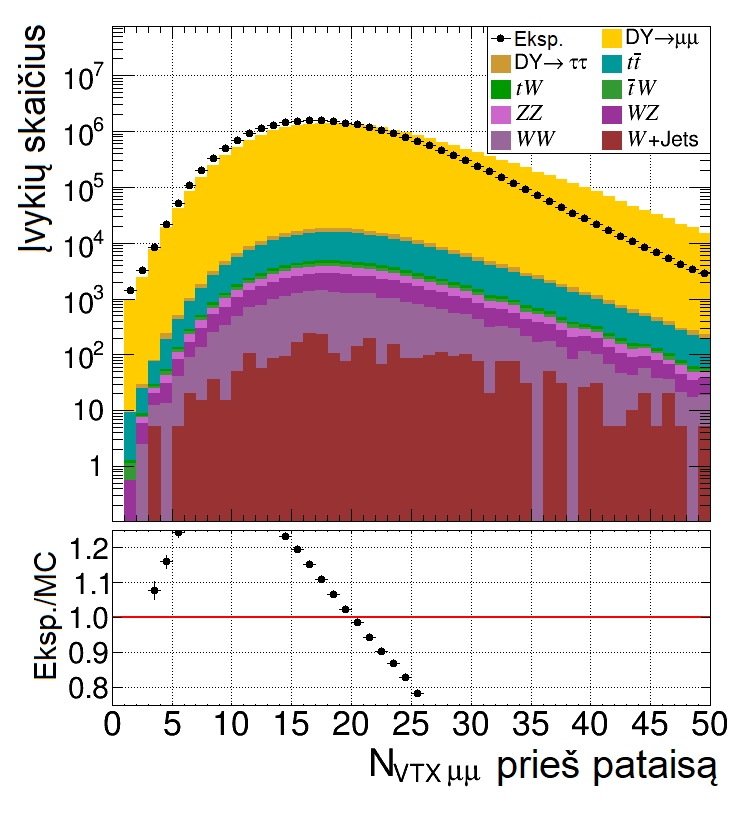
\includegraphics[width=0.48\textwidth]{Kursinis3/mumu_nVTX_before.png}
	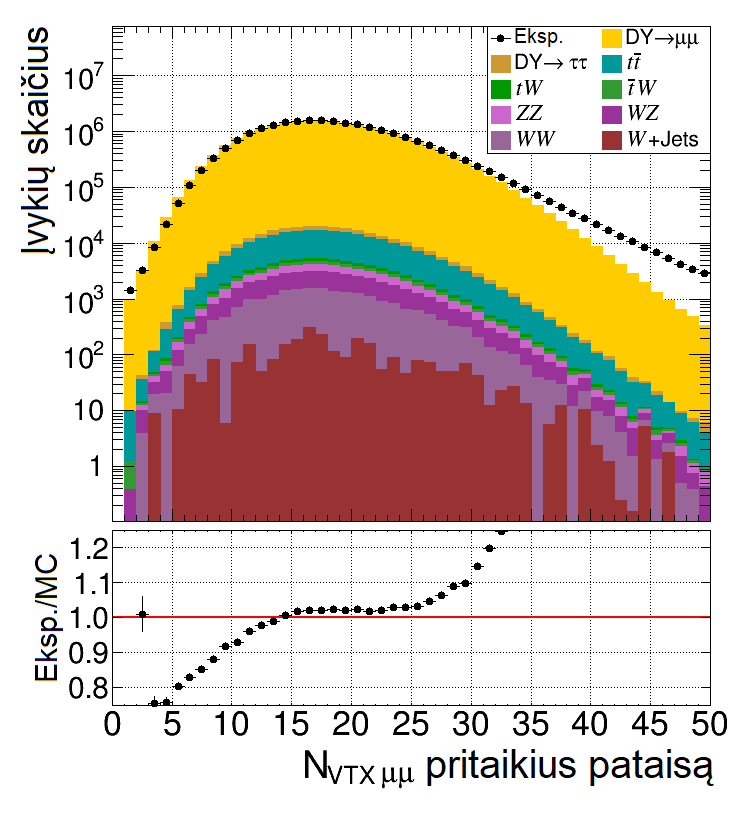
\includegraphics[width=0.48\textwidth]{Kursinis3/mumu_nVTX_after.png}
	\caption{\label{fig:PUba} Pirminių viršūnių skaičiaus pasiskirstymai atranką praėjusiuose įvykiuose prieš (kairėje)
		ir po (dešinėje) protonų susidūrimų tankio pataisos pritaikymo.
		Juodi taškai vaizduoja CMS detektoriumi išmatuotą, o spalvoti stulpeliai -- modeliuotus pasiskirstymus.}
\end{figure}

Miuonų poros invariantinės masės matavimo kokybei ženklios įtakos turi miuonų skersinio impulso matavimo tikslumas.
Dėl šios priežasties visiems užregistruotiems miuonams buvo pritaikytos Ročesterio mokslinės grupės pateikiamos
miuonų impulso matavimo skalės pataisos \cite{RocCorr}.

Dėl modeliavimo netobulumo dažnai nesutampa tam tikros realaus ir virtualaus eksperimento sąlygos.
Kiekvienam miuonų poros įvykiui buvo priskiriami svoriniai daugikliai, priartinantys modeliuotus trigerio
suveikimo bei miuono trajektorijos atkūrimo, atpažinimo ir izoliuotumo įvertinimo efektyvumus prie išmatuotųjų verčių.
Kiekvieno suvidurkinto daugiklio vertė buvo nustatoma pagal leptono skersinio impulso ir pseudospartos vertes.
Tipinė svorinio daugiklio vertė yra apie $0.9$.
Invariantinės masės pasiskirstymai prieš ir po šių pataisų pritaikymo pateikiami atitinkamai \ref{fig:invMba} pav.
Pritaikius minėtas pataisas sutapimas tarp eksperimento ir modeliavimo pagerėjo vidutiniškai apie $10\%$.

Yra pastebėta, kad pirmos eilės perturbacijų tikslumu modeliuojant viršūninių kvarkų poros ($t\bar{t}\,$)
įvykius, gaunami skersinių impulsų pasiskirstymai turi nesutapimų su nustatytaisiais eksperimentiškai \cite{ttbarPT}.
Juos buvo bandoma ištaisyti modeliuotiems viršūninių kvarkų poros įvykiams priskiriant viršūninio kvarko tyrimo grupės
siūlomus svorius, kurie skirti priartinti modeliuotą skersinių impulsų pasiskirstymą prie naujausių eksperimentinių rezultatų.
Svorių vertės nustatomos pagal kvarkų skersinių impulsų $p_{\mathrm{T}}^{t}$ vertes.
Tipinės svorių vertės yra didesnės už $1$, kai abiejų kvarkų $p_{\mathrm{T}}^{t}<123 \, \mathrm{GeV}$, ir mažesnės už $1$,
kai $p_{\mathrm{T}}^{t}>120 \, \mathrm{GeV}$.

\begin{figure}[H]
	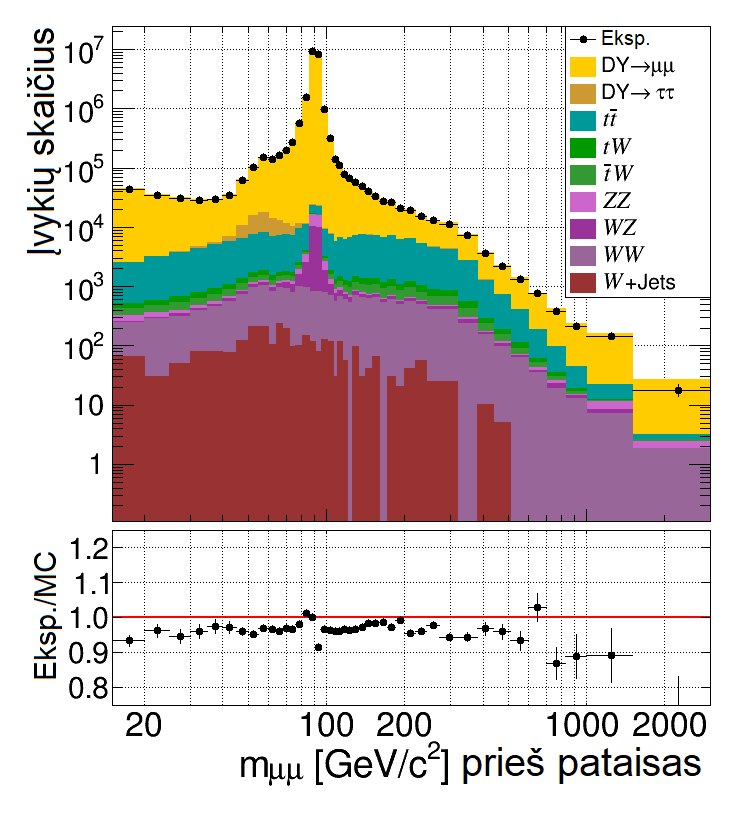
\includegraphics[width=0.48\textwidth]{Kursinis3/mumu_mass_before.png}
	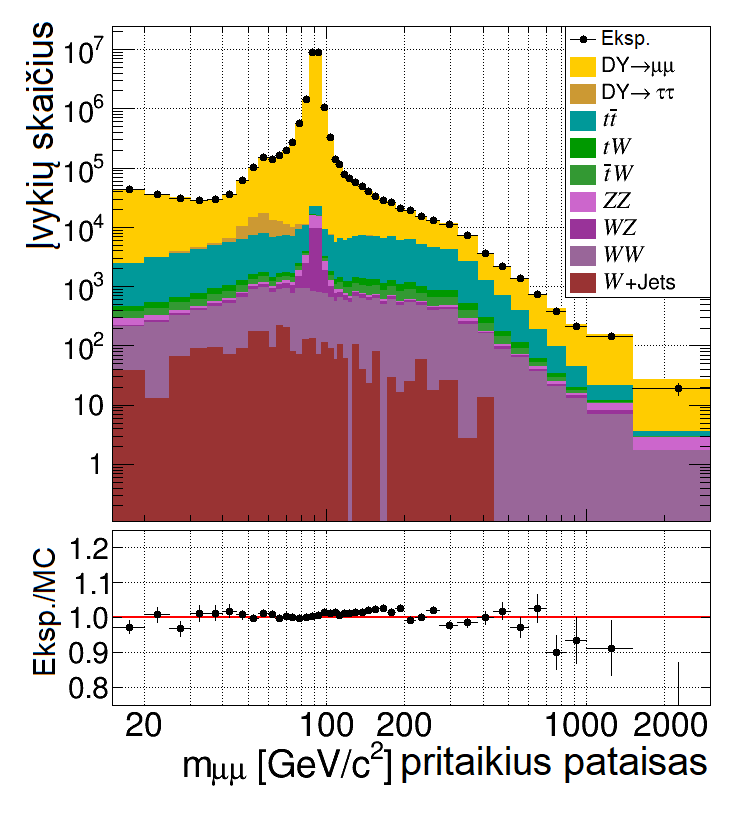
\includegraphics[width=0.48\textwidth]{Kursinis3/mumu_mass_afterSF.png}
	\caption{\label{fig:invMba} Miuonų porų invariantinės masės pasiskirstymai prieš ir po miuonų impulso matavimo skalės
	bei efektyvumo pataisų pritaikymo.}
\end{figure}

Matavimo ir modeliavimo rezultatų nesutapimą gali nulemti ne tik modeliavimo trūkumai, bet ir neidealios eksperimentinės sąlygos
arba eksperimentatorių klaidos.
Leptonų poros spartos pasiskirstymus paveikė dvi aplinkybės, į kurias buvo bandoma atsižvelgti pritaikant dar dvi pataisas.
Viena pataisa buvo skirta ištaisyti protonų susidūrimo vietos $z$ koordinatės ($z$ ašis eina išilgai protonų
spindulio lėkimo krypties detektoriaus centre) nesutapimą tarp matavimo ir modeliavimo.
Tai padėjo sumažinti matavimo ir modeliavimo santykio pasiskirstymuose buvusius asimetriškumus tarp teigiamų ir neigiamų leptonų
poros spartos verčių.
Antroji pataisa buvo reikalinga todėl, kad eksperimento duomenų registravimo laikotarpiu buvo susidurta su problema,
kai dėl laiko matavimo netikslumo trigerio suveikimas kartais buvo priskiriamas ne tam įvykiui, kuris iš tikrųjų jį aktyvavo, o
ankstesniam.
Dėl šio efekto dalis įdomių įvykių, kuriuose sukurtos dalelės turėjo dideles pseudospartos vertes ($|\eta|>2$) liko neįrašyti.
Imituoti šiam pernelyg ankstyvo trigerio suveikimo efektui buvo pritaikyta pataisa, kuri priskirdavo įvykiams
svorius pagal tai, kiek ir kokių įvykyje užregistruotų objektų patenka į dideių pseudospartų sritį.
Ši pataisa turėjo įtakos ir leptonų poros spartos pasiskirstymui.
Ji padėjo sumažinti modeliuotų įvykių skaičių prie didesnių spartos modulio verčių.
Tipinės pataisos vertės vienam įvykiui siekė apie $0.98$ ir mažiau, jeigu jame buvo užfiksuota objektų, kurių $|\eta|>2$.
Taip modeliuotas rezultatas buvo priartintas prie išmatuotojo.
\ref{fig:rapiba} pav.\ pavaizduoti leptonų poros spartos pasiskirstymai prieš ir po abiejų minėtų pataisų pritaikymo.

\begin{figure}[H]
	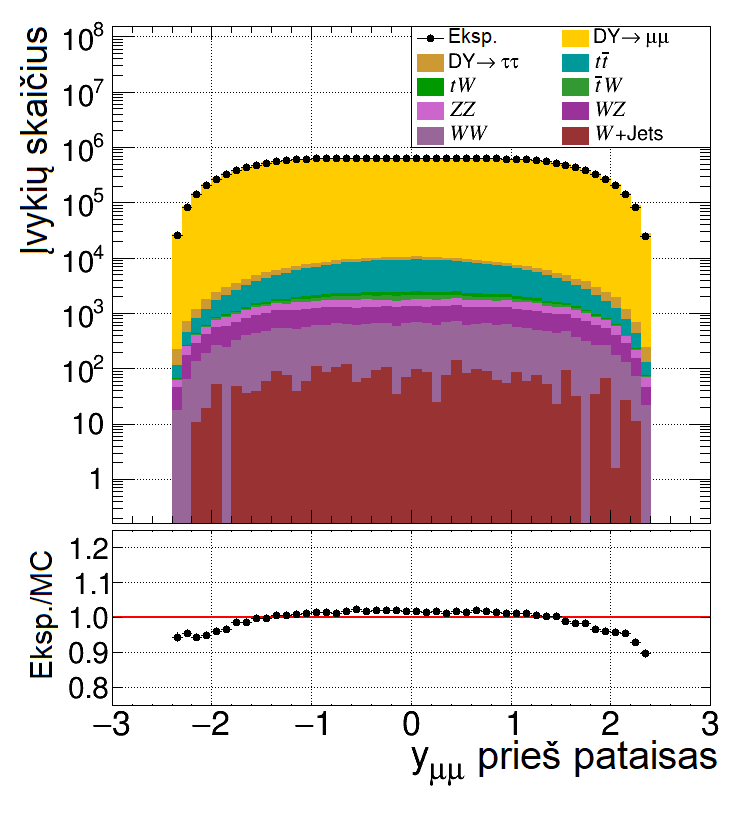
\includegraphics[width=0.48\textwidth]{Kursinis3/mumu_rapi_beforePVz.png}
	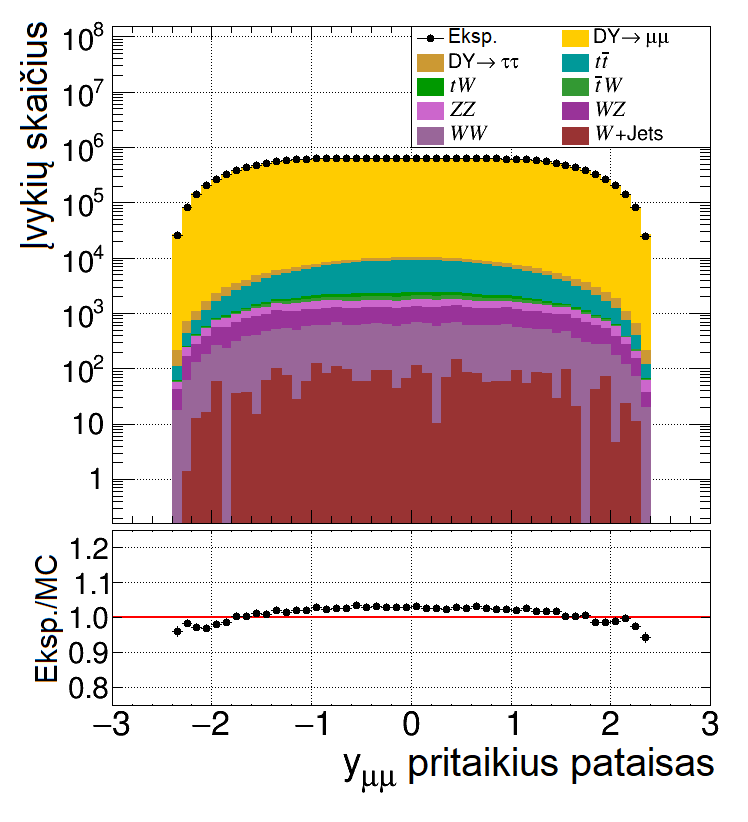
\includegraphics[width=0.48\textwidth]{Kursinis3/mumu_rapi_after.png}
	\caption{\label{fig:rapiba} Miuonų porų spartos pasiskirstymai prieš ir po pirminės viršūnės $z$ koordinatės bei per ankstaus
	trigerio suveikimo pataisų pritaikymo.}
\end{figure}

\subsection{Matavimu grįsti metodai Drell-Yan proceso triukšmo įvykių skaičiaus įvertinimui}
Matavimu grįstų metodų esmė -- nustatyti triukšmo įvykių skaičių kontrolinėje srityje, kurioje triukšmas dominuoja
ir gautą rezultatą transformuoti į signalo sritį, kuri yra tiriama.
Trumpas matavimu grįsto $\emu$ metodo aprašymas buvo pateiktas ankstesniame skyriuje, o čia bus plačiau aptariamas
klaidingo fizikinio objekto atpažinimo metodas, kuris buvo taikomas šiame darbe.
Klaidingo fizikinio objekto atpažinimo metodu buvo įvertintas $\WJets$ ir $\QCD$ procesų indėlis.
$\DYtau$, $t\bar{t}\,$, $WW$, $tW$ ir $\bar{t}W$ triukšmo procesų indėlis buvo įvertintas $\emu$ metodu ankstesniame darbe.
$WZ$ ir $ZZ$ įvykių skaičius buvo įvertintas iš modeliavimo.

\subsubsection{Klaidingo atpažinimo metodas}

Klaidingo fizikinio objekto atpažinimo metodas buvo naudojamas įvertinti skaičiui tokių triukšmo įvykių, kuriuose čiurkšlės
buvo atpažintos, kaip miuonai: $\WJets$ ir $\QCD$.
Signalo ir kontrolinė sritys buvo apibrėžtos pagal miuono trajektorijos izoliuotumą: miuonai su $I_{\mathrm{PF}}^{\mathrm{rel.}}<0.15$
priskiriami signalo sričiai, o visi kiti ($I_{\mathrm{PF}}^{\mathrm{rel.}} \geqslant 0.15$) -- kontrolinei sričiai.

\paragraph{Klaidingo atpažinimo tikimybės įvertinimas\\}

Įvykiai klaidingo atpažinimo tikimybei įvertinti buvo atrenkami pagal \ref{table:FR} lentelėje nurodytus atrankos kriterijus.
Drell-Yan signalo atrankoje naudoti vieno miuono trigeriai šiuo atveju buvo netinkami, nes juose yra užkoduotas ir miuono trajektorijos
izoliuotumo reikalavimas, kuris šiuo atveju buvo nereikalingas.
Dėl šios priežasties buvo pasirinktas kitas vieno miuono trigeris, kuris aktyvuojamas, kai aptinkamas miuonas su skersiniu impulsu,
viršijančiu $50$ GeV. Šis trigeris neatsižvelgia į miuono izoliuotumą.
Dėl pasikeitusio trigerio buvo naudojami ir kitokie kinematiniai reikalavimai: atrenkami miuonai su $\pT>52$ GeV.
Miuonams buvo taikomas tas pats Drell-Yan signalo atrankoje naudotas \ttt{TightID} reikalavimas.
Reikalavimai miuono krūviui ar įvykyje užregistruotų miuonų skaičiui nebuvo taikomi.
Klaidingo atpažinimo tikimybė buvo įvertinta pagal \ref{eq:realfake} formulę keliose skirtingose miuono skersinio impulso ir
pseudospartos srityse ($f_{\mathrm{Signal} \, | \, \mathrm{Jet}}$ yra funkcija nuo $\pT$ ir $\eta$).

\begin{table}
	\begin{tabular}{|c|c|}
		\hline
		\textbf{Signalo sritis} & \textbf{Kontrolinė sritis} \\
		\hline\hline
		\multicolumn{2}{|c|}{Trigeris \ttt{Mu\_50}} \\
		\hline
		\multicolumn{2}{|c|}{$\pT>52$ GeV} \\
		\hline
		\multicolumn{2}{|c|}{$|\eta|<2.4$} \\
		\hline
		\multicolumn{2}{|c|}{\ttt{TightID} reikalavimai} \\
		\hline
		$I_{\mathrm{PF}}^{\mathrm{rel.}} < 0.15$ & $I_{\mathrm{PF}}^{\mathrm{rel.}} > 0.15$ \\
		\hline
	\end{tabular}
	\caption{\label{table:FR} Naudoti miuonų atrankos kriterijai signalo ir kontrolinei sritims. Visi kriterijai, išskyrus vieną
	abiem sritims yra vienodi.}
\end{table}

Minėtą įvykių atranką praeina ir įvykiai, kuriuose miuonai yra tikri, todėl, norint teisingai įvertinti klaidingo atpažinimo
tikimybę, iš eksperimento metu užregistruotų duomenų reikėjo išskirti $\QCD$ proceso įvykius.
$\QCD$ įvykių išskyrimui buvo pasitelkti modeliuoti duomenų rinkiniai.
Paprasčiausias variantas išskirti $\QCD$ įvykius būtų iš atranką praėjusių eksperimento metu užregistruotų įvykių skaičiaus
atėmus modeliuotą visų su $\QCD$ nesusijusių procesų įvykių skaičių:
\begin{multline}
	N^{\QCD}_{i} = N^{\mathrm{Data}}_{i} - \left( N^{\mathrm{DY}}_{i} +
	N^{W+\mathrm{Jets}}_{i} + N^{\ttbar}_{i} + N^{tW+\tbarW}_{i} +
	N^{WW+WZ+ZZ}_{i} \right)^{\mathrm{MC}}; \\ i = \mathrm{signal}, \, \mathrm{control},
\end{multline}
tačiau šis metodas nėra tinkamas, nes pašalinių įvykių skaičius yra pakankamai didelis, o taip pat įvykiai, kuriuose leptonai
nėra izoliuoti, yra prasčiau sumodeliuoti ir ne taip gerai sutampa su matavimu.
Tikslesniam $\QCD$ įvykių skaičiaus įvertinimui buvo naudojami du skirtingi metodai:
\begin{enumerate}
	\item Santykio metodas -- $\QCD$ įvykių skaičius įvertinamas iš matavimo paėmus procentinę $QCD$ įvykių dalį, kuri buvo apskaičiuota
	pasinaudojant modeliavimu:
	\begin{multline}
		N^{\QCD}_{i} = N^{\mathrm{Data}}_{i} \cdot \left(\frac{N^{\QCD}_{i}}
		{N^{\QCD}_{i} + N^{\mathrm{DY}}_{i} + N^{W+\mathrm{Jets}}_{i} +
		N^{\ttbar}_{i} + N^{tW+\tbarW}_{i} + N^{WW+WZ+ZZ}_{i}} \right)^{\mathrm{MC}}; \\ i = \mathrm{signal}, \, \mathrm{control}.
	\end{multline}
	\item Šablonų pritaikymo (angl. \textit{template fitting}) metodas -- $\QCD$ įvykių skaičius įvertinamas prie tam tikro
	išmatuoto pasiskirstymo pritaikius skirtingų procesų pasiskirstymų šablonus.
	Skirtingų procesų šablonai dažniausiai (ir šiuo atveju) gaunami iš modeliavimo.
	Pasiskirstymas, kurio šablonai pritaikomi prie matavimo, turi būti pasirenkamas toks, kuris leistų pakankamai gerai
	atskirti $\QCD$ nuo kitų procesų (pasiskirstymų forma turėtų būti skirtinga).
	Šiuo atveju buvo naudojami miuono trajektorijos izoliuotumo pasiskirstymo šablonai.
	Turint detektoriaus išmatuotą pasiskirstymą ir skirtingų procesų šablonus, stengiamasi gauti geriausią sutapimą tarp matavimo ir
	šablonų sumos varijuojant kiekvienam šablonui priskirtus svorinius daugiklius:
	\begin{multline}
		N^{\mathrm{Data}}_{i}(I^{\mathrm{rel.}}_{\mathrm{PF}}) \approx
		\lambda^{\mathrm{fit}}_{\,i}\, N^{\,\QCD}_{i}(I^{\mathrm{rel.}}_{\mathrm{PF}}) +
		\epsilon^{\,\mathrm{fit}}_{\,i}\, N^{\,\mathrm{DY}}_{i}(I^{\mathrm{rel.}}_{\mathrm{PF}}) +
		\zeta^{\,\mathrm{fit}}_{\,i}\, N^{\,W+\mathrm{Jets}}_{i}(I^{\mathrm{rel.}}_{\mathrm{PF}}) +
		\theta^{\,\mathrm{fit}}_{i}\, N^{\,\ttbar}_{i}(I^{\mathrm{rel.}}_{\mathrm{PF}}) + \\[7pt] +
		\kappa^{\,\mathrm{fit}}_{\,i}\, N^{\,tW}_{i}(I^{\mathrm{rel.}}_{\mathrm{PF}}) + 
		\xi^{\,\mathrm{fit}}_{i}\, N^{\,\tbarW}_{i}(I^{\mathrm{rel.}}_{\mathrm{PF}}) +
		\tau^{\,\mathrm{fit}}_{i}\, N^{\,WW}_{i}(I^{\mathrm{rel.}}_{\mathrm{PF}}) +
		\chi^{\,\mathrm{fit}}_{\,i}\, N^{\,W\!Z}_{i}(I^{\mathrm{rel.}}_{\mathrm{PF}}) +
		\psi^{\,\mathrm{fit}}_{i}\, N^{\,Z\!Z}_{i}(I^{\mathrm{rel.}}_{\mathrm{PF}}); \\ i = \mathrm{signal}, \, \mathrm{control}.
	\end{multline}
	Čia $\lambda^{\mathrm{fit}}_{\,i}$, $\epsilon^{\,\mathrm{fit}}_{\,i}$ ir t.t.\ -- varijuojami daugikliai,
	kuriuos keičiant bandoma gauti geriausią šablonų sumos sutapimą su matavimu mažiausių kvadratų metodu.
	Idealiu atveju šie daugikliai turėtų būti lygūs vienetui. 
	Gavus daugiklių vertes klaidingo atpažinimo tikimybė įvertinama naudojant modeliuotą $\QCD$ įvykių skaičių, padaugintą
	iš gautojo daugiklio vertės:
	\begin{equation}
		f_{\mathrm{signal} \,| \,\mathrm{Jet}} =
		\frac{\lambda^{\mathrm{fit}}_{\,\mathrm{signal}}\, N^{\,\QCD \; \mathrm{MC}}_{\mathrm{signal}}}
		{\lambda^{\mathrm{fit}}_{\,\mathrm{signal}}\, N^{\,\QCD \; \mathrm{MC}}_{\mathrm{signal}} +
		\lambda^{\mathrm{fit}}_{\,\mathrm{control}}\, N^{\,\QCD \; \mathrm{MC}}_{\mathrm{control}}}\, .
	\end{equation}
	Svarbu atkreipti dėmesį, kad, nors šablonų pritaikymas daromas izoliuotumo pasiskirstymui, šis pasiskirstymas klaidingo
	atpažinimo tikimybėje neatsispindi: įvertindami klaidingo atpažinimo tikimybę naudojame tik gautą svorinio daugiklio vertę.
	Šiame darbe šablonų pritaikymas, panašiai kaip ir pats klaidingo atpažinimo tikimybės įvertinimas buvo atliekamas keliose
	skirtingose miuono skersinio impulso ir pseudospartos srityse.
	Šablonų pritaikymo metodas yra laikomas tikslesniu, nei santykio metodas, todėl jis buvo naudojamas kaip pagrindinis rezultatas.
\end{enumerate}


\paragraph{Klaidingo atpažinimo tikimybės pritaikymas triukšmo įvykių skaičiaus įvertinimui\\}

$\QCD$ ir $\WJets$ triukšmo įvykių skaičiaus įvertinimui buvo vykdoma įvykių atranka, kurios kriterijai nurodyti
\ref{table:jetSelection} lentelėje.
Praktiškai visi taikyti atrankos kriterijai buvo identiški Drell-Yan signalo atrankos kriterijams, nurodytiems
\ref{table:selection} lentelėje, tačiau vienam arba dviems miuonams buvo taikomi invertuoti trajektorijos izoliuotumo
reikalavimai (atitinkamai $\WJets$ arba $\QCD$ atrankoje).
Taip pat šiuo atveju nebuvo naudojamas joks aukšto lygio trigeris, nes, norint teisingai įvertinti triukšmo įvykių skaičių
svarbu, kad taikomi kinematiniai reikalavimai atitiktų naudojamus pagrindinėje analizėje.
To nebūtų įmanoma padaryti naudojant klaidingo atpažinimo tikimybės įvertinimui naudotą trigerį trigerį \ttt{Mu\_50},
o pagrindinės analizės trigeriai taip pat buvo netinkami dėl jau minėto reikalavimo miuonų izoliuotumui.
Smarkaus skaičiavimo laiko išaugimo dėl trigerio nenaudojimo buvo išvengta iškart atmetant visus įvykius, kuriuose nebuvo
užfiksuota bent dviejų miuonų.

\begin{table}
	\begin{tabular}{|c|c|}
		\hline
		\textbf{$\WJets$ atranka} & \textbf{$\QCD$ atranka} \\
		\hline\hline
		\multicolumn{2}{|c|}{Trigeris: --} \\
		\hline
		\multicolumn{2}{|c|}{$p_{\mathrm{T \, 1}} > 28$ GeV, $p_{\mathrm{T \, 2}} > 17$ GeV} \\
		\hline
		\multicolumn{2}{|c|}{$|\eta_1| < 2.4$, $|\eta_2| < 2.4$} \\
		\hline
		\multicolumn{2}{|c|}{\ttt{TightID} reikalavimai} \\
		\hline
		\multicolumn{2}{|c|}{\multirow{3}{17em}{\centering Pasirenkami 2 miuonai, kuriuos galima tiksliausiai suvesti į vieną
		pirminę viršūnę su $\chi^2<20$}} \\
		\multicolumn{2}{|c|}{} \\
		\multicolumn{2}{|c|}{} \\
		\hline
		\multicolumn{2}{|c|}{Priešingi elektriniai krūviai} \\
		\hline
		\multicolumn{2}{|c|}{Plokštuminis kampas $< \pi - 0.005$ rad} \\
		\hline
		\multirow{2}{15em}{\centering Vienam miuonui $I_{\mathrm{PF}}^{\mathrm{rel.}}<0.15$,
			kitam -- $I_{\mathrm{PF}}^{\mathrm{rel.}}\geqslant 0.15$} &
			\multirow{2}{15em}{\centering Abiems miuonams $I_{\mathrm{PF}}^{\mathrm{rel.}}\geqslant 0.15$} \\
		 & \\
		\hline
	\end{tabular}
	\caption{\label{table:jetSelection}Apibendrinti $\WJets$ ir $\QCD$ įvykių atrankos kriterijai. Indeksai $1$ ir $2$ žymi
	atitinkamai greitesnįjį ir lėtesnįjį miuoną. Šios dvi atrankos skiriasi tik vienu kriterijumi.}
\end{table}

$\QCD$ įvykių skaičiaus įvertinimui gautos klaidingo atpažinimo tikimybės vertės buvo pritaikytos naudojantis \ref{eq:FRQCD}
formule.
Praktiškai tai buvo įgyvendinta kiekvienam įvykiui priskiriant svorinį daugiklį $\frac{ff}{(1-f)(1-f)}$ pagal tai, kokie
yra įvykyje užregistruotų miuonų skersiniai impulsai ir pseudospartos.
\ref{table:jetSelection} lentelėje nurodytus atrankos kriterijus praeina ne vien tik $\QCD$ įvykiai, tačiau jų yra pakankamai
nedaug, kad iš matavimo būtų galima paprasčiausiai atimti modeliuotus kitų procesų įverčius.

Klaidingo atpažinimo tikimybė $\WJets$ įvykių skaičiaus įvertinimui buvo pritaikyta naudojantis \ref{eq:FRWjets} formule.
Šiuo atveju įvykiams buvo pritaikomi svoriniai daugikliai $\frac{f}{1-f}$ pagal tai, koks yra neizoliuoto miuono skersinis
impulsas ir pseudosparta.
Lyginant su $\QCD$ įvykių atranka, $\WJets$ atranką praeina gerokai daugiau su $\WJets$ nesusijusių įvykių
(ypatingai Drell-Yan proceso įvykių), todėl šiuo atveju įvertinti $\WJets$ įvykių skaičių atimant modeliuotą įvykių skaičių
iš eksperimento metu užregistruoto nėra optimalu.
$\WJets$ įvykių skaičius buvo įvertintas panaudojus šablonų pritaikymą.
Šįkart buvo naudojami leptonų poros invariantinės masės pasiskirstymo (t.y., ieškomo pasiskirstymo) šablonai.
Drell-Yan ir $\ttbar$ procesams buvo naudojami modeliuoti šablonai, $\QCD$ procesui buvo naudojamas klaidingo atpažinimo
metodu įvertintas šablonas, o $\WJets$ šablonas buvo gautas iš miuonų porų, kurios praeitų $\WJets$ atranką, tačiau
miuonai yra vienodo elektrinio krūvio.
Vienodo krūvio pasiskirstyme dominuoja $\WJets$ įvykiai, todėl ten $\WJets$ pasiskistymą galima įvertinti tiesiog iš matavimo
atėmus sumodeliuotus pašalinius procesus.
Vienodo krūvio $\WJets$ šabloną galima naudoti kaip priešingo krūvio, nes šių procesų kinematika turėtų nesiskirti (skiriasi
tik tikimybės sukurti vienodų arba skirtingų krūvių $W$ bozoną ir čiurkšlę), taigi pasiskirstymai turėtų turėti apytiksliai
vienodą formą, bet skirtingą suintegruotą įvykių skaičių.
Įvykių skaičiaus klausimą šiuo atveju išsprendė šablonų pritaikymas.


\subsection{Paklaidų įvertinimas}\label{sec:uncertainties}

Analizuojant protonų susidūrimus laikoma, įvykių skaičius yra pasiskirstęs pagal Puasono dėsnį.
Puasono pasiskirstymu aprašomo įvykių skaičiaus standartinis nuokrypis yra lygus kvadratiniai šakniai iš labiausiai
tikėtino įvykių skaičiaus.
Atliekant realų eksperimentą, labiausiai tikėtinas įvykių skaičius nėra tiksliai žinomas, todėl atranką praėjusių
įvykių skaičiaus statistinio neapibrėžtumo verte laikoma kvadratinė šaknis iš užregistruoto įvykių skaičiaus.

Kai modeliuoti įvykiai turi nelygius vienetui svorius, jų skaičiaus $N$ statistinis neapibrėžtumas $(\Delta N)_{\mathrm{Stat.\,}}$
įvertinamas kaip kvadratinė šaknis iš modeliuotų įvykių svorių kvadratų sumos:
\begin{equation}
	(\Delta N)_{\mathrm{Stat.\,}} = \sqrt{\sum_{i=1}^{N}w_{i}^{2}} \; ,
	\label{eq:Sumw2Unc}
\end{equation}
čia $$w_{i}=w_{i}^{\mathrm{Norm.}} \cdot \prod_{p=1}^{N_{\mathrm{Pat.}}}w_{i}^{p} \; ,$$
kur $w_{i}^{\mathrm{Norm.}}$ -- modeliuoto įvykio normuojantis svoris, gaunamas iš \ref{eq:NLOweight} išraiškos,
$w_{i}^{p}$ -- modeliuotam įvykiui pataisos $p$ priskirtas svorinis daugiklis, $N_{\mathrm{Pat.}}$ -- pritaikytų
skirtingų pataisų skaičius.
Jeigu modeliuotų įvykių turime daugiau, nei buvo užregistruota eksperimento metu, jiems bus priskiriami mažesni už
vienetą svoriai ir sunormuoto įvykių skaičiaus statistinė paklaida bus mažesnė nei eksperimento metu užregistruotų
įvykių.
Tai yra vienas iš modeliavimo privalumų, kai modeliuojami mažo tikėtinumo įvykiai.
Tuo tarpu, kai modeliuojami labai didelio tikėtinumo įvykiai, jiems priskiriami svoriai taip pat būna labai dideli
ir statistinis neapibrėžtumas bus gerokai didesnis nei detektoriaus užregistruotų įvykių.
Tai yra vienas iš modeliavimo trūkumų ir viena iš pagrindinių priežasčių, kodėl naudojamas klaidingo atpažinimo metodas
$\QCD$ ir $\WJets$ įvykių skaičiaus įvertinimui -- jų reakcijos skerspjūviai yra labai dideli ir norint juos kokybiškai
sumodeliuoti reikia ypatingai didelių skaičiavimo resursų.
Jeigu įvykiams priskiriami vienetui lygius svoriai, iš \ref{eq:Sumw2Unc} išraiškos gauname, kad įvykių
skaičiaus paklaida lygi kvadratinei šakniai iš įvykių skaičiaus, taigi, ši formulė tinkama ir eksperimento
metu užregistruotų įvykių skaičiaus statistinio neapibrėžtumo įvertinimui.

Jeigu įvykių skaičius yra išvestinis dydis jo neapibrėžtumas apskaičiuojamas pasinaudojant šia išraiška:

\begin{equation}
	\Delta f(x, y, ...) =
	\sqrt{ \left( \frac{\partial f}{\partial x} \Delta x \right)^{2} +
	\left( \frac{\partial f}{\partial y} \Delta y \right)^{2} + ... } \;\; \mathrm{,}
	\label{eq:DerUnc}
\end{equation}
čia $x$ ir $y$ -- nepriklausomi dydžiai.
Klaidingo fizikinio objekto atpažinimo metodu įvertinto triukšmo įvykių skaičiaus statistinis neapibrėžtumas taip
pat buvo įvertintas paimant kvadratinę šaknį iš gauto rezultato, nes klaidingo atpažinimo tikimybė yra naudojama
kaip svorinis daugiklis, kuris bendru atveju yra labai mažas, todėl neapibrėžtumas, įvertintas naudojantis
\ref{eq:Sumw2Unc} formule yra netikroviškai mažas.
% PATIKRTINTI ŠITĄ TEIGINĮ!!!

Galimiems sisteminiams nukrypimams įvertinti CMS statistikos komitetas rekomenduoja turėti bent du skirtingais būdais
atliktus matavimus, kurie, idealiu atveju, turėtų duoti sutampančius įverčius.
Kadangi tikroji vertė, kurią bandoma išmatuoti, yra nežinoma, daroma prielaida, jog skirtingi įverčiai yra
lygiaverčiai ir nepriklausomi, o tikroji vertė yra artimoje aplinkoje.
Tokiu atveju skirtumo tarp dviejų skirtingų rezultatų absoliučioji vertė yra pakankamai saugus sisteminės matavimo
paklaidos įvertis.

Šiame darbe buvo matuojamas Drell-Yan proceso triukšmo įvykių skaičius, o turimi du skirtingi įverčiai buvo gauti naudojant
skirtingas klaidingo atpažinimo tikimybės įvertinimo metodikas: santykio ir šablonų pritaikymo metodą.
Taigi, pagrindinė $\QCD$ ir $\WJets$ įvykių skaičiaus įverčio sisteminės paklaidos sudedamoji dalis buvo įvertinta pagal
tokią formulę:
\begin{equation}
	(\Delta N_{ll}^{\mathcal{P} \; \mathrm{įvert.}})_{\mathrm{Sist.\,}} =
	\left| N_{ll}^{\mathcal{P} \; \mathrm{įvert.}}(\mathrm{fit.}) -
	N_{ll}^{\mathcal{P} \; \mathrm{įvert.}}(\mathrm{sant.}) \right| \;  ;
	\;\;\;\;\; \mathcal{P} = \QCD, \; \WJets \; ,
	\label{eq:systUncFR}
\end{equation}
čia \ltq{įvert.} žymi matavimu grįstą įvertį, \ltq{fit.} žymi klaidingo atpažinimo tikimybei įvertinti naudotą šablonų
pritaikymo metodą, o \ltq{sant.} -- santykio metodą.

Kadangi klaidingo atpažinimo tikimybei įvertinti buvo naudojamas baigtinis įvykių skaičius, ji turi savo statistinį neapibrėžtumą,
kuris neatsispindi galutinio triukšmo įvykių skaičiaus įverčio statistiniame neapibrėžtume.
Dėl šios priežasties klaidingo atpažinimo tikimybės statistinis neapibrėžtumas buvo įskaitomas laikant jį papildomu indėliu į
sisteminę įverčio paklaidą.
Skirtingos paklaidos dedamosios, laikant, kad jos yra tarpusavyje nepriklausomos, buvo sudedamos pagal Pitagoro teoremą.

\section{Rezultatai ir jų aptarimas}

Drell-Yan proceso triukšmo įvykių skaičius, susijęs su $\DYtau$, $t\bar{t}\,$, $WW$, $tW$, $\bar{t}W$ procesais buvo įvertintas
$\emu$ metodu ankstesniame darbe.
Šie triukšmo įvykiai sudaro $1.06\%$ visų $\mu\mu$ įvykių.
Triukšmo įvykių skaičiaus įvertis buvo gautas taikant \eqref{eq:emuMethod} formulę kiekvienam miuonų poros invariantinės masės
histogramos stulpeliui atskirai.
Statistinės įvykių skaičiaus paklaidos buvo įvertintos naudojantis \eqref{eq:Sumw2Unc} ir \eqref{eq:DerUnc}.
Sisteminė $\emu$ metodo įverčio paklaida buvo įvertinta kaip skirtumo tarp modeliuoto ir $\emu$ metodo įverčio modulis, pagal
CMS statistikos komiteto rekomendacijas.
Suminės paklaidos gautos susumavus statistinę ir sisteminę paklaidas pagal Pitagoro teoremą.
Invariantinės masės histogramų, kai naudojami vien modeliuoti įverčiai ir kai naudojamas $\emu$ metodas palyginimas pateikiamas
\ref{fig:MassMCemu} pav.
Modeliuotų $\mu\mu$ triukšmo įvykių skaičius lygus $250500$, o įvertinus $\mu\mu$ triukšmo įvykių skaičių  $e\mu$ metodu
gauta $241105$ įvykių.
Lyginant su modeliavimu, $\emu$ metodas visoje tirtoje invariantinės masės srityje susumuotą triukšmo įvykių skaičių
sumažino maždaug $4$-ais procentais.
Abiejuose pateikiamuose grafikuose naudojami modeliuoti $WZ$, $ZZ$ ir $W+\mathrm{Jets}$ procesų įverčiai.
Modeliuotas $\QCD$ įvertis grafikuose nepateikiamas dėl labai prastos modeliavimo kokybės.

\begin{figure}[H]
	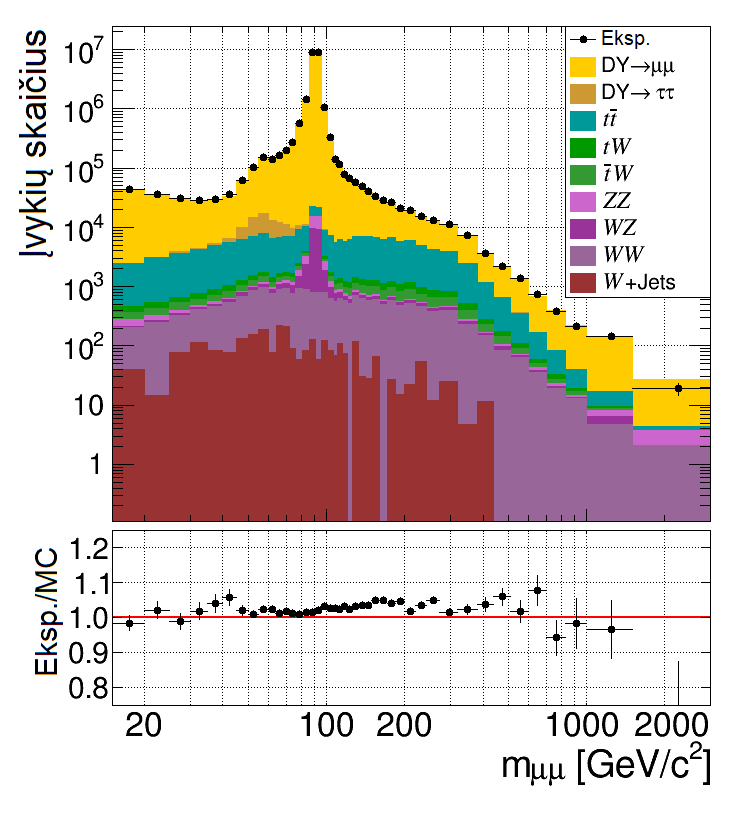
\includegraphics[width=0.49\textwidth]{Kursinis3/mumu_mass_after.png}
	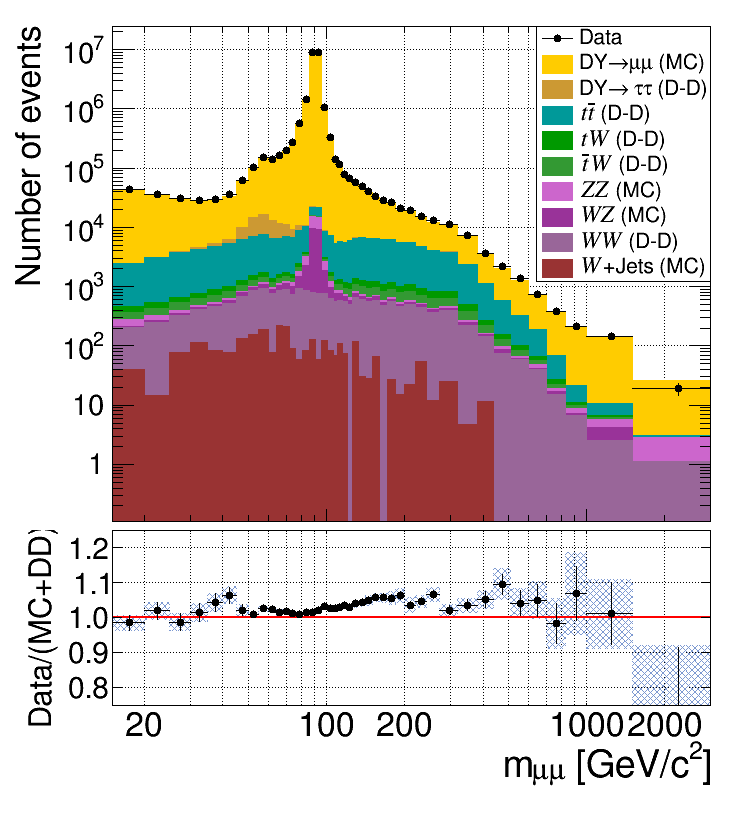
\includegraphics[width=0.49\textwidth]{Kursinis3/mumu_mass_wEMuEst.png}
	\caption{\label{fig:MassMCemu}
		Miuonų poros invariantinės masės pasiskirstymai pritaikius visas pataisas.
		Juodi taškai vaizduoja CMS detektoriumi išmatuotus pasiskirstymus, o spalvoti stulpeliai -- modeliuotus (kairėje)
		arba $\emu$ metodu įvertintus (dešinėje) įvykius.
		Eksperimento ir įverčio santykio grafike esančios mėlynos juostos vaizduoja sumines paklaidas.}
\end{figure}

Įvykių atranka miuono klaidingo atpažinimo tikimybės įvertinimui buvo atlikta taikant \ref{table:FR} lentelėje išvardintus
kriterijus.
\ref{fig:jet_pT_before} pav.\ pavaizduoti atranką praėjusių miuonų skersinio impulso pasiskirstymai.
Dėl nepakankamai tikslaus modeliavimo nesutapimas tarp eksperimento ir modeliavimo siekia $20\%$.
Dėl šios priežasties buvo laikoma, jog klaidingo atpažinimo tikimybės įvertinimas naudojant santykio metodą gali būti
nepakankamai teisingas.
Kokybiškesnį įvertinimą buvo tikimasi gauti naudojant šablonų pritaikymo metodą.
Jis buvo atliekamas prie matavimo pritaikant modeliuotus miuono trajektorijos izoliuotumo pasiskirstymus.
Izoliuotumo pasiskirstymai buvo padalinti į šešias sritis: pirmiausia dalinama į dvi dalis pagal miuono pseudospartą
($|\eta|<1.2$ atitinka miuonus, pataikiusius į detektoriaus cilindrinę dalį, o $|\eta|\geqslant 1.2$ -- į antgalių segmentus)
bei į tris dalis pagal miuono skersinį impulsą ($52<\pT<70$, $70\leqslant \pT<100$ ir $100\leqslant \pT<500$).
Prie išmatuotų izoliuotumo pasiskirstymų pritaikyti šablonai pavaizduoti \ref{fig:templateFit} pav.
Šablonų pritaikymas pakoregavo modeliuotų pasiskirstymų normavimą taip, kad nesutapimas tarp matavimo ir modeliavimo
sumažėjo iki $5\%$.
Pernormuoti miuonų skersinio impulso pasiskirstymai pavaizduoti \ref{fig:jet_pT_after} pav.
Klaidingo atpažinimo tikimybė buvo įvertinta skirtingose miuono skersinio impulso srityse bei dviejose pseudospartos srityse
(atitinkančiose detektoriaus cilindro ir antgalių segmentus) naudojantis \ref{eq:FR} formule.
Klaidingo atpažinimo tikimybės vertės, gautos naudojant santykio ir šablonų pritaikymo metodus, pavaizduotos \ref{fig:FR} pav.
Šablonų pritaikymo metodu gautos klaidingo atpažinimo tikimybės vertės yra beveik $10\%$ didesnės, už įvertintas
santyskio metodu.
Čiurkšlės, pataikiusios į detektoriaus antgalį klaidingo atpažinimo tikimybė yra vidutiniškai $2.5$ karto didesnė už
čiurkšlės, pataikiusios į cilindrinę dalį.

Apskaičiuota klaidingo atpažinimo tikimybė buvo panaudota įvertinant Drell-Yan proceso triukšmo įvykių skaičių, susijusį su
$\QCD$ ir $\WJets$ procesais.
Triukšmo įvykių skaičiaus įvertinimui reikalingų įvykių atranka buvo vykdoma pagal \ref{table:jetSelection} lentelėje
išvardintus kriterijus.
$\QCD$ įvykių skaičius iš kontrolinės į signalo sritį buvo perkeliamas atranką praėjusiems įvykiams pritaikius svorinius
daugiklius, apskaičiuojamus pagal \ref{eq:FRQCD} formulę.
\ref{fig:QCDselection} pav.\ pateiktas atranką praėjusių į signalo sritį perkeltų miuonų porų pasiskirstymas.
Modeliavimas sufleruoja, kad tokią įvykių atranką praeina ne tik $\QCD$ proceso įvykiai, tačiau pašaliniai įvykiai
sudaro tik apie $25\%$ viso įvykių skaičiaus.
$\QCD$ įvykių skaičius buvo gautas iš eksperimento metu išmatuoto pasiskirstymo atėmus modeliuotus pasiskirstymus.
Įverčio rezultatas pavaizduotas \ref{fig:QCDest} pav.
Taigi, įvertintas su $\QCD$ procesu susijusių Drell-Yan proceso triukšmo įvykių skaičius yra lygus $2884\pm 54$.

\begin{figure}[H]
	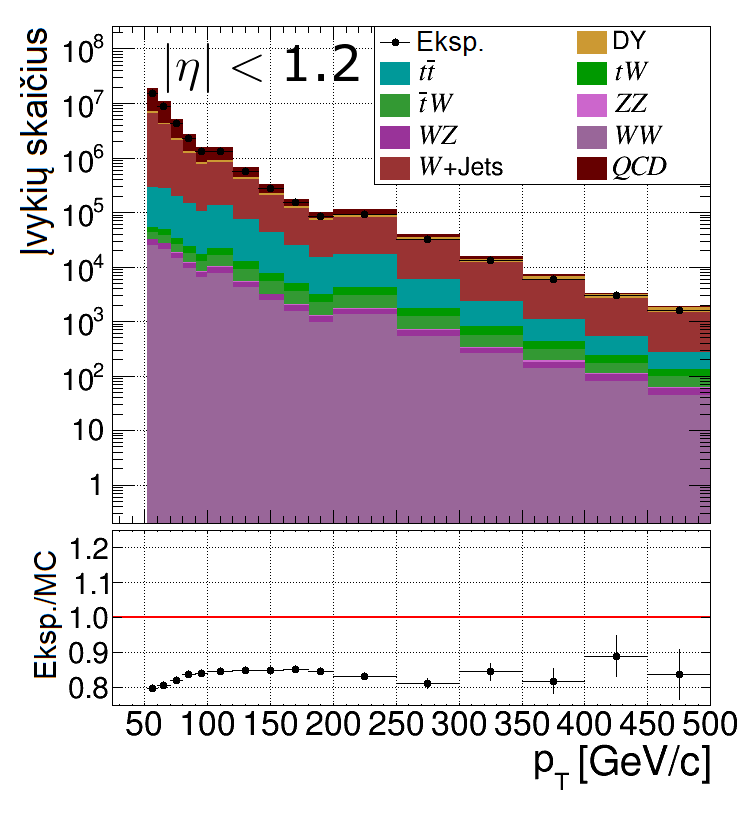
\includegraphics[width=0.48\textwidth]{Kursinis3/FRest_pT_deno_barrel.png}
	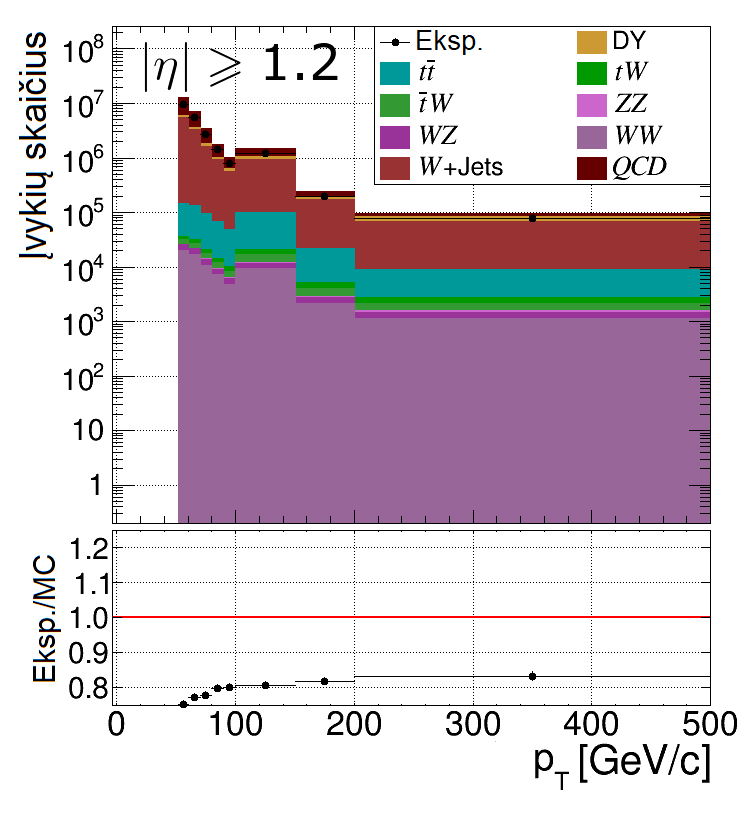
\includegraphics[width=0.48\textwidth]{Kursinis3/FRest_pT_deno_endcap.png}
	\caption{\label{fig:jet_pT_before}
		Klaidingo atpažinimo tikimybės įvertinimui atliktą įvykių atranką praėjusių miuonų kandidatų skersinių impulsų
		pasiskirstymai, kai miuonas pataiko į detektoriaus cilindrinę (kairėje) ir antgalio (dešinėje) dalį.
		Dėl nepakankamai tikslaus modeliavimo, jo sutapimas su eksperimento rezultatu yra prastas.}
\end{figure}

\begin{figure}[H]
	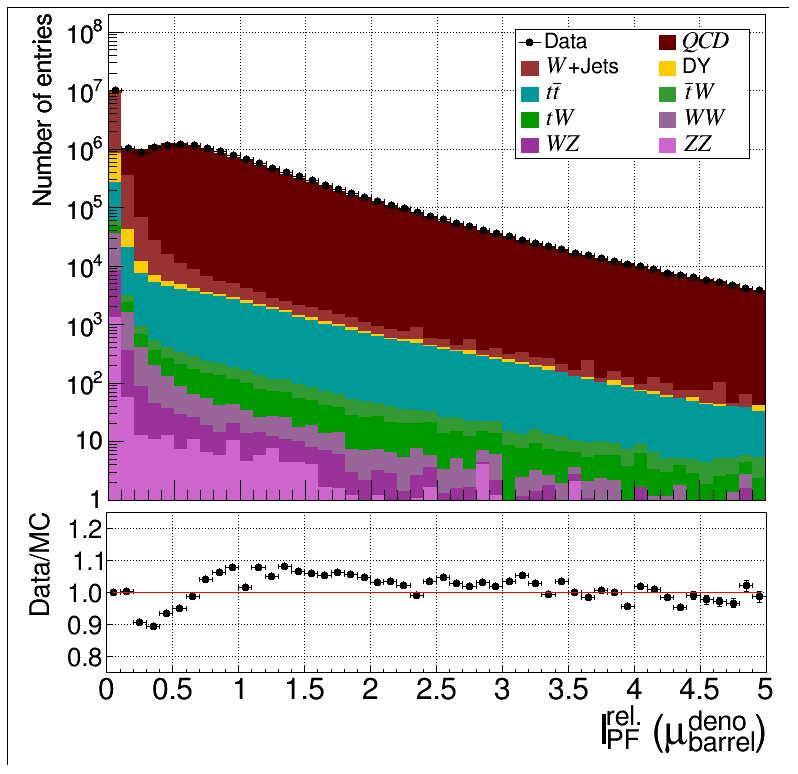
\includegraphics[width=0.45\textwidth]{Kursinis3/TFit_DB_50to70.png}
	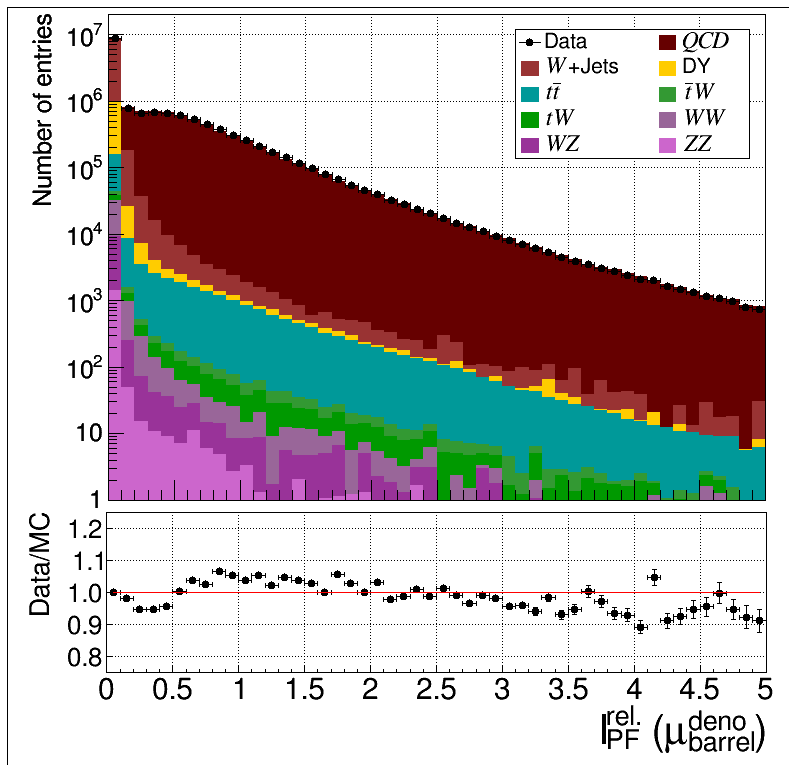
\includegraphics[width=0.45\textwidth]{Kursinis3/TFit_DE_50to70.png}
	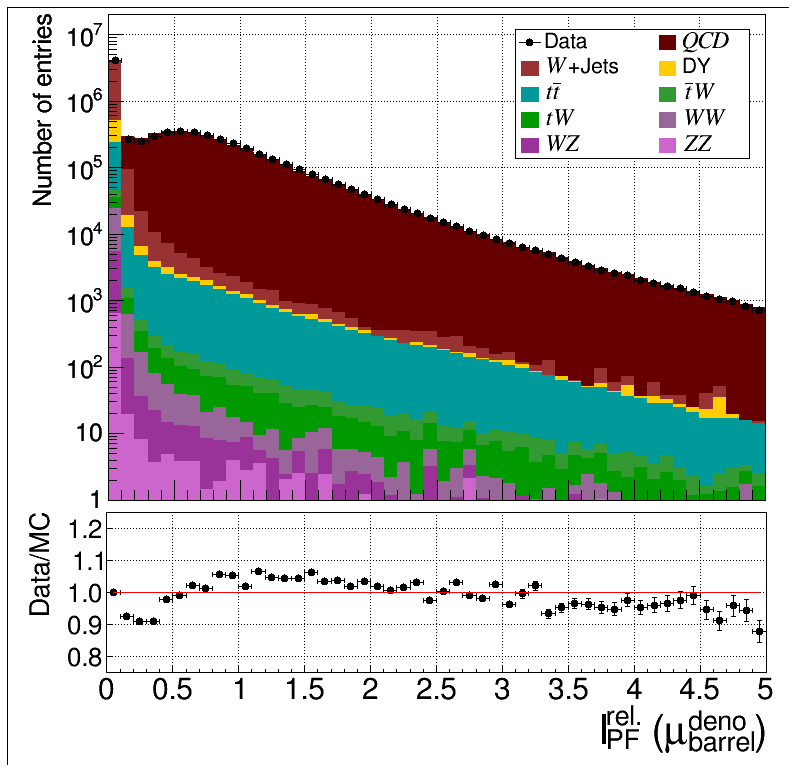
\includegraphics[width=0.45\textwidth]{Kursinis3/TFit_DB_70to100.png}
	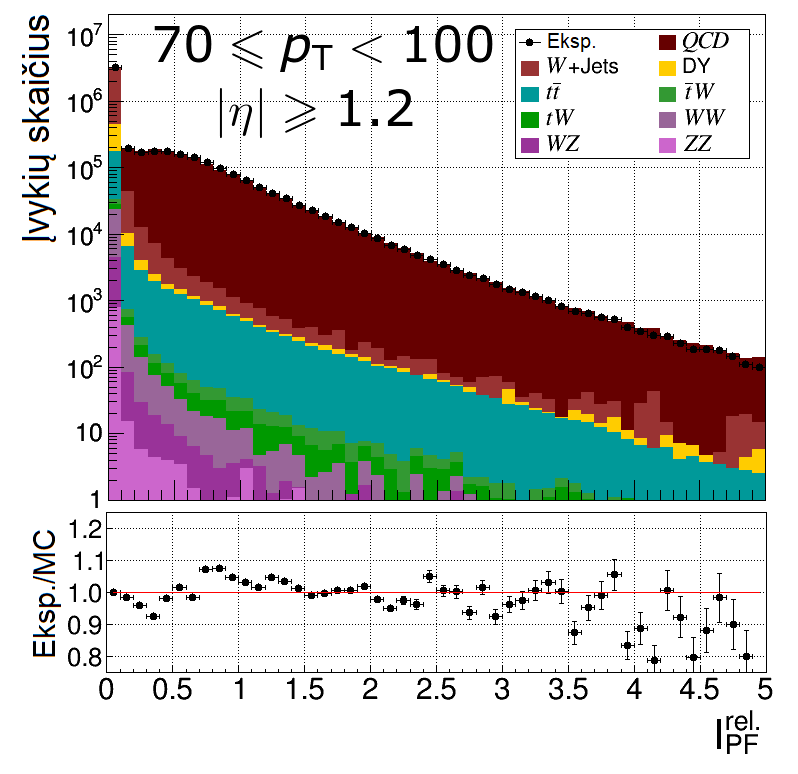
\includegraphics[width=0.45\textwidth]{Kursinis3/TFit_DE_70to100.png}
	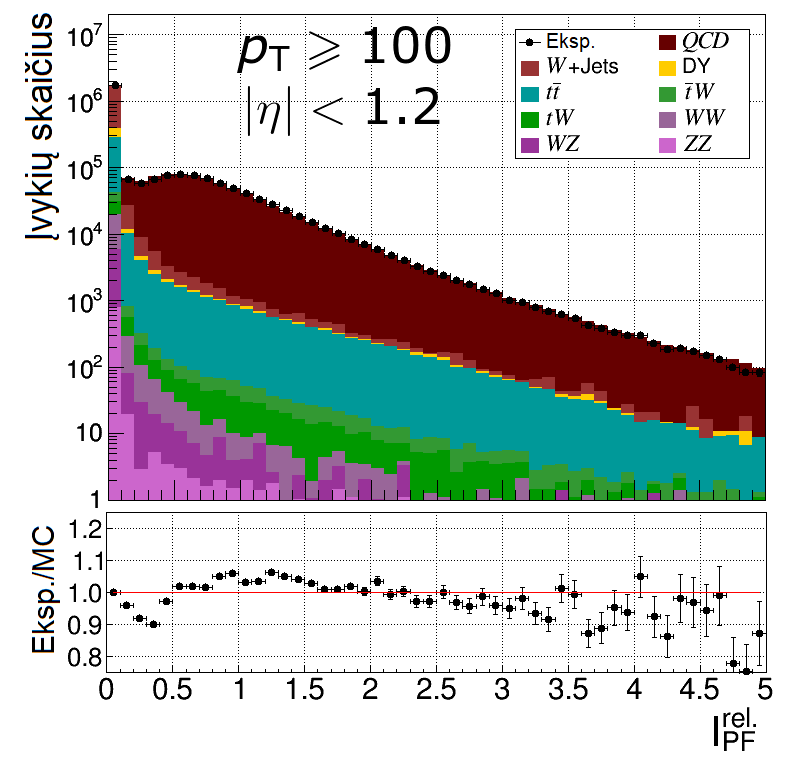
\includegraphics[width=0.45\textwidth]{Kursinis3/TFit_DB_100to500.png}
	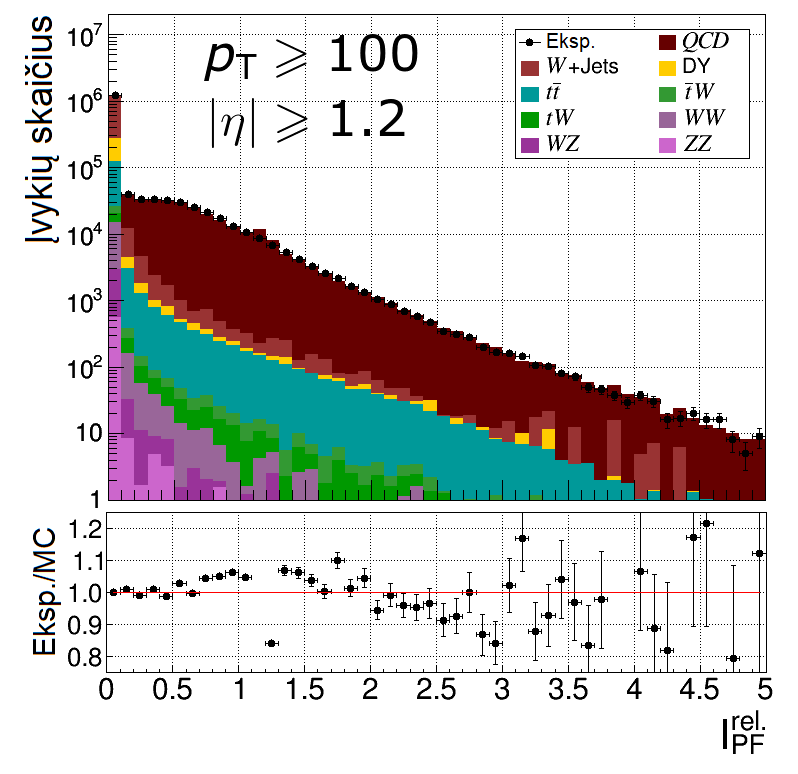
\includegraphics[width=0.45\textwidth]{Kursinis3/TFit_DE_100to500.png}
	\caption{\label{fig:templateFit}
		Eksperimentiniai miuono trajektorijos izoliuotumo pasiskirstymai detektoriaus cilindrinėje (kairėje)
		ir  antgalių (dešinėje) dalyse, bei prie jų pritaikyti modeliuoti šablonai.
		Iš viršaus į apačią pavaizduoti pasiskirstimai miuonų kandidatams, kurių $\pT\in(52, 70)$,
		$\pT\in[70, 100)$ ir $\pT\in[100, 500)$.}
\end{figure}

\begin{figure}[H]
	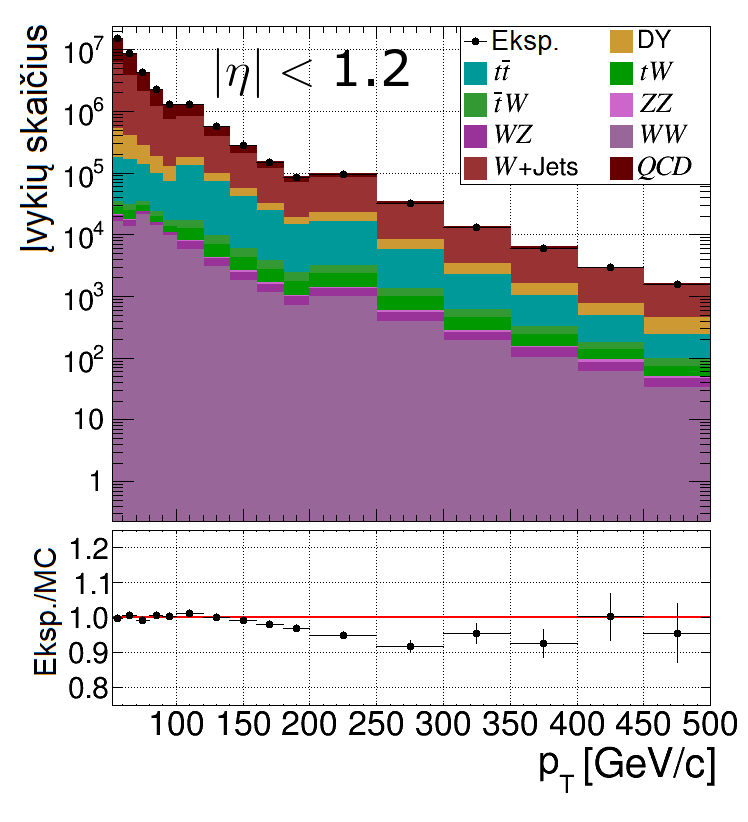
\includegraphics[width=0.48\textwidth]{Kursinis3/FRfit_pT_deno_barrel.png}
	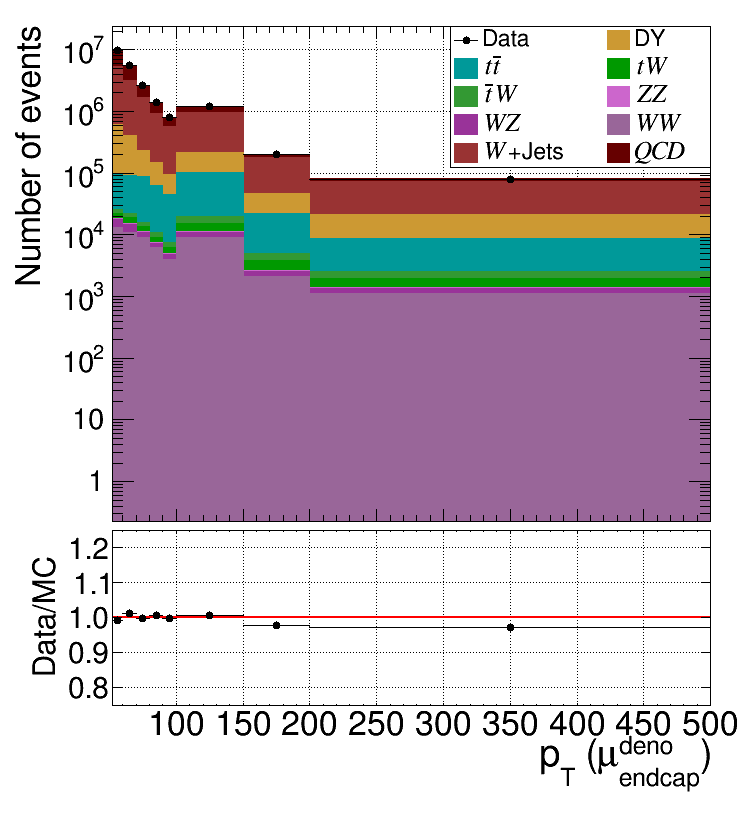
\includegraphics[width=0.48\textwidth]{Kursinis3/FRfit_pT_deno_endcap.png}
	\caption{\label{fig:jet_pT_after}
		Klaidingo atpažinimo tikimybės įvertinimui atliktą įvykių atranką praėjusių miuonų kandidatų skersinių impulsų
		pasiskirstymai, kai miuonas pataiko į detektoriaus cilindrinę (kairėje) ir antgalio (dešinėje) dalį.
		Šiuose grafikuose modeliuoti pasiskirstymai yra pernormuoti, kad atitiktų iš šablonų pritaikymo gautas vertes.}
\end{figure}

\begin{figure}[H]
	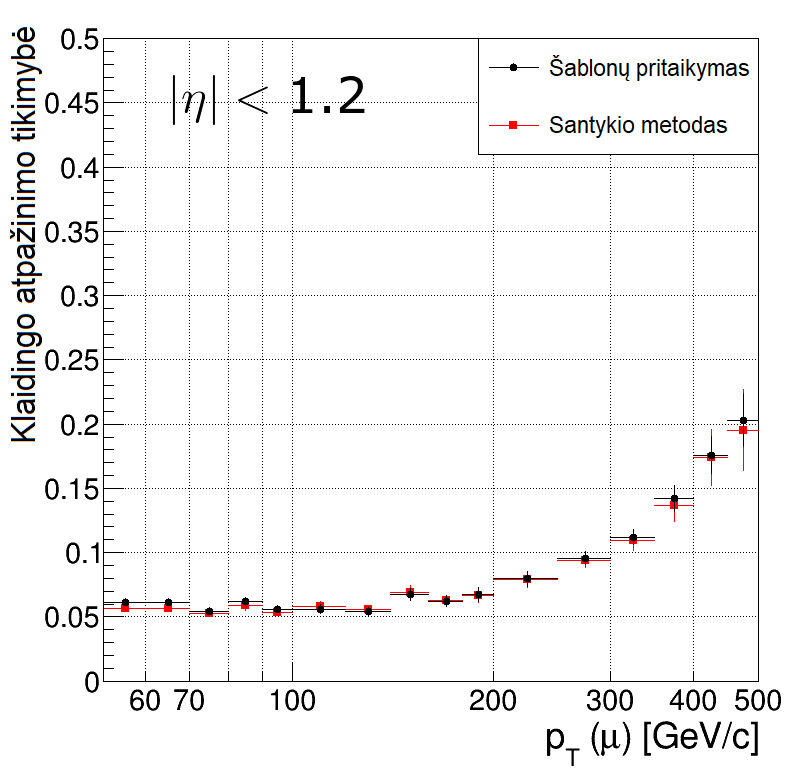
\includegraphics[width=0.48\textwidth]{Kursinis3/FR_barrel.png}
	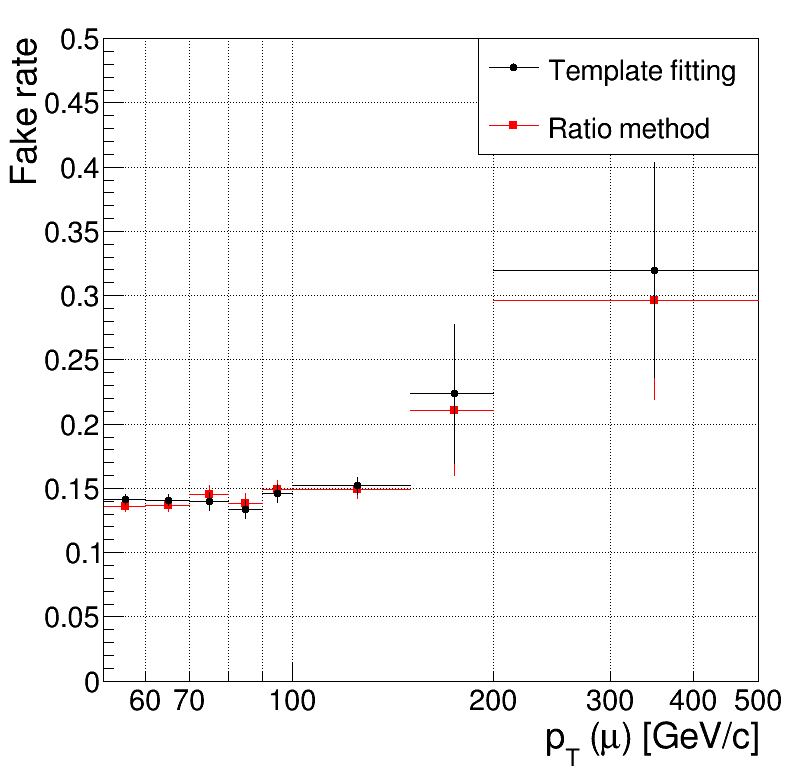
\includegraphics[width=0.48\textwidth]{Kursinis3/FR_endcap.png}
	\caption{\label{fig:FR}
		Apskaičiuota klaidingo atpažinimo tikimybė skirtingose skersinio impulso srityse.
		Kairėje pateiktas rezultatas trajektorijoms, einančioms per detektoriaus cilindinę, o dešinėje -- per antgalių dalis.
		Skirtingos spalvos vaizduoja skirtingais metodais įvertintą tikimybę (žr. legendą).}
\end{figure}

\begin{minipage}{0.47\textwidth}
	\centering
	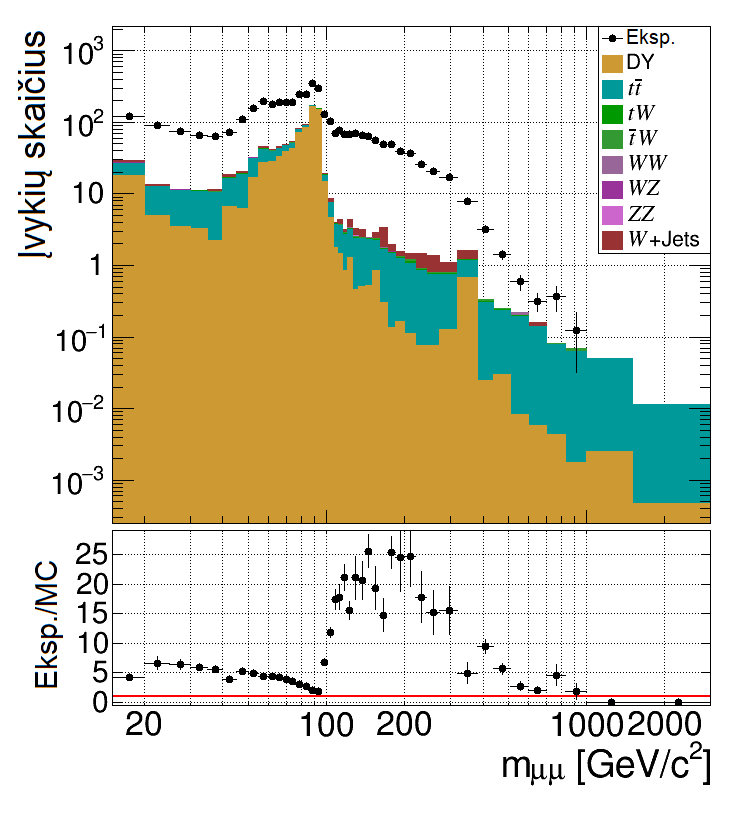
\includegraphics[width=0.98\textwidth]{Kursinis3/QCDest_subtract.png}
	\vspace{-0.5cm}
	\captionof{figure}{\label{fig:QCDselection}
		$\QCD$ įvykių atranką praėjusių į signalo sritį perkeltų miuonų kandidatų porų invariantinės masės pasiskirstymas.
		Spalvotais stulpeliais pavaizduoti modeliuoti su $\QCD$ procesu nesusiję pasiskirstymai, kurie buvo atimami iš
		išmatuotojo pasiskirstymo.
	}
\end{minipage}
\hfill
\begin{minipage}{0.45\textwidth}
	\centering
	\vspace{-1.5cm}
	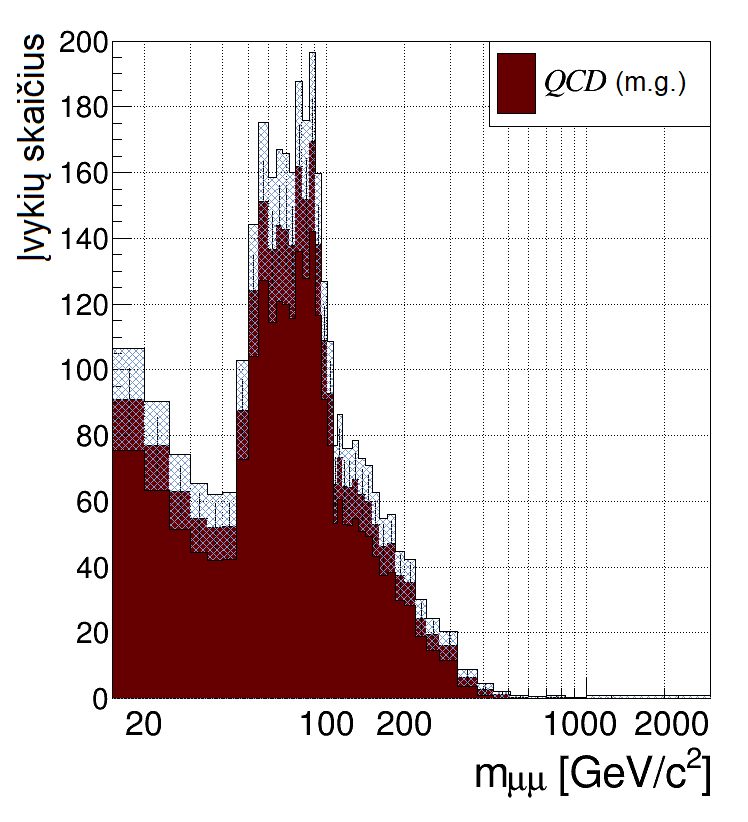
\includegraphics[width=0.98\textwidth]{Kursinis3/QCDest.png}
	\captionof{figure}{\label{fig:QCDest}
		Klaidingo atpažinimo metodu įvertintas $\QCD$ proceso indėlis į Drell-Yan proceso atranką praeinančių miuonų
		porų invariantinės masės pasiskirstymą.
	}
\end{minipage}
\vspace{0.5cm}

$\WJets$ įvykių skaičius iš kontrolinės į signalo sritį buvo perkeliamas atranką praėjusiems įvykiams pritaikius svorinius
daugiklius pagal \ref{eq:FRWjets} formulę.
Skirtingai nei $\QCD$ atranką, $\WJets$ atranką praeina didelė dalis pašalinių procesų: net $84.5\%$ visų įvykių yra
nesusiję su $\WJets$.
Modeliavimas sufleruoja, kad didžiausią indėlį į įvykių skaičių turi Drell-Yan ir $\ttbar$ procesai.
Tokiu atveju iš išmatuotojo pasiskirstymo atimti modeliuotą nėra tinkama procedūra, tad $\WJets$ pasiskirstymas buvo
gautas pasinaudojus šablonų pritaikymu.
Šiuo atveju šablonai buvo pritaikomi prie į signalo sritį perkeltų $\WJets$ atranką praėjusių miuonų porų invariantinės
masės pasiskirstymo.
$\WJets$ pasiskirstymo šablonas buvo gautas iš $\WJets$ atranką praėjusių vienodo krūvio miuonų pasiskirstymo,
kuris yra mažiau užterštas su Drell-Yan proceso įvykiais.
Vienodo krūvio $\WJets$ pasiskirstymą galima naudoti kaip šabloną priešingo krūvio pasiskirstymui, nes čiurkšlėje įmanoma pagaminti
bet kokio krūvio miuoną ir vidutinė proceso kinematika nuo miuono krūvio neturėtų priklausyti.
Turėtų skirtis tik šių procesų tikimybės.
Iš modeliavimo buvo įvertinta, kad priešingo krūvio $\WJets$ įvykiai yra maždaug 3 kartus dažnesni, nei vienodo krūvio.
$\QCD$ proceso šablonas buvo gautas panaudojant klaidingo atpažinimo metodu įvertintą $\QCD$ pasiskirstymą.
Kitiems procesams buvo naudojami modeliuoti šablonai.
\ref{fig:TFit_WJets} pav.\ pateiktas šablonų pritaikymo rezultatas.
Iš šablonų pritaikymo gautas $\WJets$ įvykių skaičius, lygus $3573 \pm 60$.
Tai yra $2.6$ kartų daugiau, nei vienodo krūvio $\WJets$ įvykių skaičius.
Su $\WJets$ procesu susijusių triukšmo įvykių indėlio įvertis pavaizduotas \ref{fig:WJetsEst} pav.
Lyginti klaidingo atpažinimo metodu gautus triukšmo įvykių pasiskirstymus su modeliuotais atitinkamų procesų įverčiais
nėra didelės prasmės, nes modeliuoti šių procesų pasiskirstymai yra smarkiai netolydūs dėl prastos statistikos.

\vspace{1cm}

\begin{minipage}{0.47\textwidth}
	\centering
	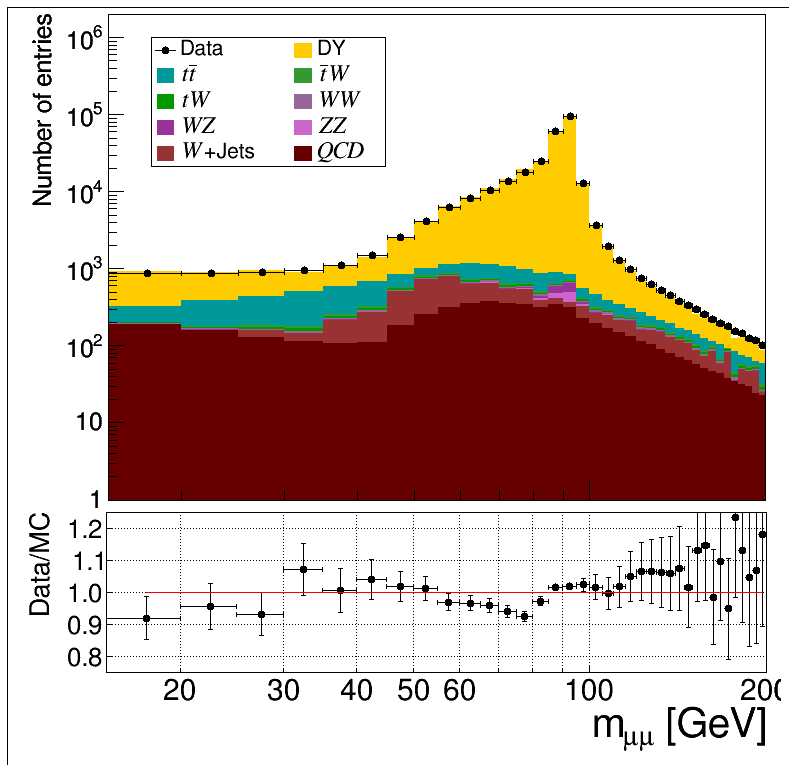
\includegraphics[width=0.98\textwidth]{Kursinis3/TFit_WJETS.png}
	\vspace{-0.3cm}
	\captionof{figure}{\label{fig:TFit_WJets}
		$\WJets$ įvykių atranką praėjusių į signalo sritį perkeltų miuonų kandidatų porų invariantinės masės pasiskirstymas
		bei prie jo pritaikyti skirtingų procesų šablonai.
	}
\end{minipage}
\hfill
\begin{minipage}{0.47\textwidth}
	\centering
	\vspace{-1.5cm}
	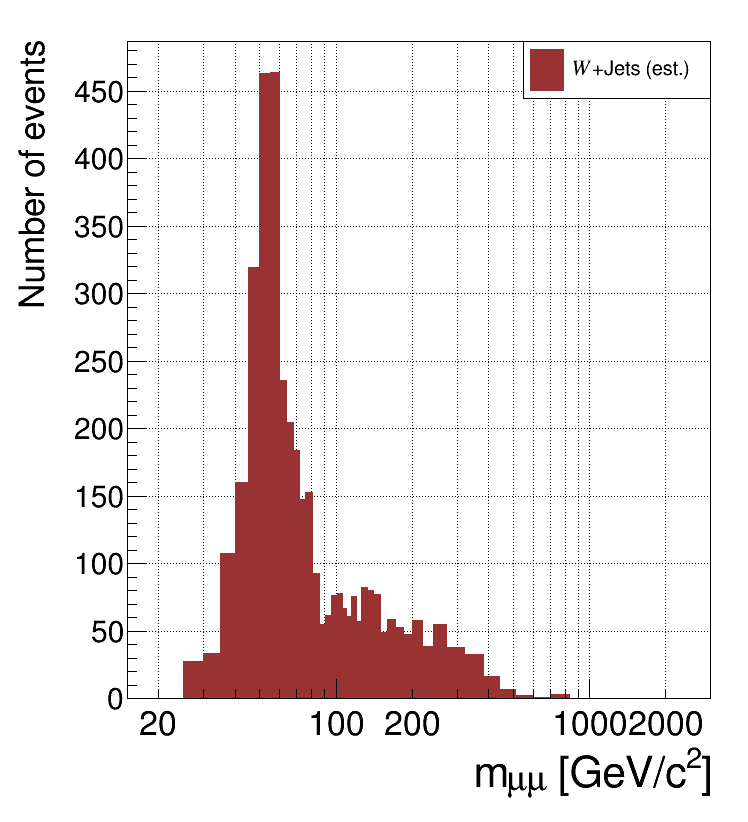
\includegraphics[width=0.98\textwidth]{Kursinis3/WJETSest.png}
	\captionof{figure}{\label{fig:WJetsEst}
		Klaidingo atpažinimo metodu įvertintas $\WJets$ proceso indėlis į Drell-Yan proceso atranką praeinančių miuonų
		porų invariantinės masės pasiskirstymą.
	}
\end{minipage}
\vspace{2cm}

Eksperimento metu išmatuoto Drell-Yan proceso atranką praėjusių miuonų porų invariantinių masių pasiskirstymo palyginimas
su susumuotais skirtingų procesų įverčiais, iš kurių tik $\WZ$ ir $\ZZ$ yra modeliuoti, yra pateiktas \ref{fig:MassFinal} pav.
Lyginant su \ref{fig:MassMCemu} pav. pateiktu grafiku, į kurį neįtraukti klaidingo fizikinio objekto atpažinimo metodo
įverčiai, sutapimas tarp matavimo ir įverčio pagerėjo $0.02\%$.
Nors pagerėjimas atrodo labai mažas, tačiau su čiurkšlėmis susiję atranką praėję įvykiai sudaro tik $0.03\%$ visų įvykių.
Beveik visi šie įvykiai kontributuoja į matavimo ir įverčio sutapimo pagerėjimą, taigi klaidingo fizikinio objekto
atpažinimo metodo taikymas buvo naudingas.

\begin{figure}[H]
	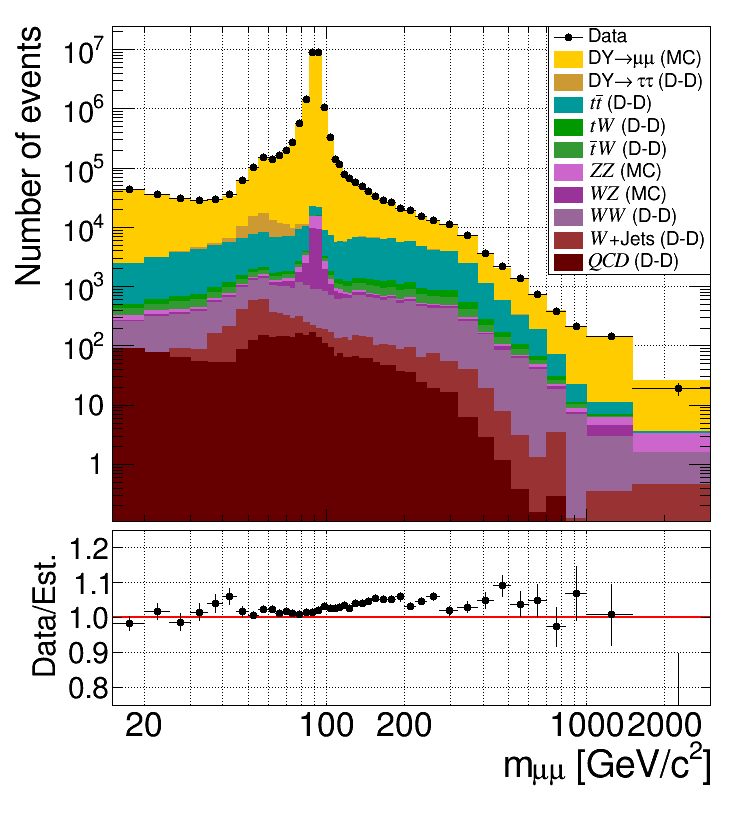
\includegraphics[width=0.48\textwidth]{Kursinis3/Mass_allEst.png}
	\vspace{-0.5cm}
	\caption{\label{fig:MassFinal}
		Eksperimento metu išmatuoto miuonų poros invariantinės masės pasiskirstymo palyginimas su matavimu grįstais
		skirtingų procesų indėlių įverčiais (išskyrus $\WZ$ ir $\ZZ$ procesų įverčius, kurie yra modeliuoti).}
\end{figure}

\section{Išvados}
\begin{enumerate}
	\item Šablonų pritaikymo metodas duoda geresnį modeliuotų pasiskirstymų sutapimą su išmatuotaisiais eksperimento metu
	nei modeliuotų įvykių normavimas pagal išmatuotą integruotąjį šviesį, todėl manoma, kad šiuo metodu įvertinta
	tikimybė čiurkšlei būti klaidingai atpažintai kaip izoliuotas miuonas yra teisingesnė.
	\item Su čiurkšlėmis susijusių Drell-Yan proceso triukšmo įvykių skaičiaus įvertis yra labai jautrus klaidingo
	fizikinio objekto atpažinimo tikimybės įvertinimo tikslumui, todėl įverčio sisteminė paklaida yra didelė.
	\commentMA{\\Turėtų būti pagrįsta grafikais ir pridėtu tekstu rezultatuose.}
	\item Dėl didelio $\WJets$ ir $\QCD$ procesų reakcijos skerspjūvio ir itin mažos tikimybės su jais susijusiems įvykiams praeiti
	Drell-Yan proceso įvykių atranką modeliuoti šių procesų įverčiai yra labai prastos kokybės.
	\item Nors klaidingo atpažinimo metodu įvertintas $\WJets$ ir $\QCD$ procesų indėlis į miuonų poros invariatinės masės
	pasiskirstymą turi nemažus neapibrėžtumus, šio įverčio kokybė yra žymiai geresnė nei modeliuoto, tad klaidingo fizikinio
	objekto atpažinimo metodo taikymas buvo naudingas.
	\commentMA{\\Į \ref{fig:MassMCemu} pav.\ įtraukti ir modeliuotą QCD pasiskirstymą ir tekste pakomentuoti, kuo ir kodėl
	modeliuoti šitų procesų įverčiai blogi.}
	\item Triukšmo įvykių skaičiaus įvertinimas klaidingo fizikinio objekto atpažinimo metodu pagerino eksperimento
	metu išmatuoto miuonų poros invariantinės masės pasiskirstymo sutapimą su skirtingų procesų įverčiais.
\end{enumerate}


%\clearpage
\section*{Santrauka}
Šiame darbe pristatomas Drell-Yan proceso triukšmo įvykių skaičiaus įvertinimas klaidingo fizikinio objekto
atpažinimo metodu.
Darbas buvo atliktas analizuojant CERN CMS eksperimento 2016 metais užregistruotus
$13$ TeV energijos protonų susidūrimų duomenis, atitinkančius $35.9$ \invfb integruotąjį šviesį.
Duomenų interpretavimui buvo pasitelkiami CMS kolektyvo paruošti modeliuoti protonų susidūrimų duomenų rinkiniai.
Drell-Yan proceso įvykių atranką praėjusiems miuonams buvo pritaikytos skersinio impulso matavimo skalės pataisos.
Modeliuotiems įvykiams buvo pritaikytas rinkinys pataisų, įskaitančių įvairius neatitikimus tarp eksperimento
ir modeliavimo sąlygų.
Įvykdžius į Drell-Yan procesą panašių įvykių atranką buvo bandoma nustatyti, koks yra triukšmo įvykių, susijusių
su klaidingai kaip miuonai atpažintomis čiurkšlėmis, skaičius.
Buvo įvertinta tikimybė, kad čiurkšlė bus klaidingai atpažinta kaip izoliuotas miuonas.
Šios tikimybės vertės buvo panaudotos įvertintant, kiek $\WJets$ (vienos čiurkšlės) ir $\QCD$ (kelių čiurkšlių)
įvykių galėjo praeiti Drell-Yan proceso įvykių atranką bei koks šių procesų indėlis į eksperimento metu
išmatuotą miuonų poros invariantinės masės pasiskirstymą.

\addcontentsline{toc}{section}{5 \hspace{0.1cm} Naudotos literatūros sąrašas}
\bibliography{KursinisDarbas}
\bibliographystyle{unsrt}

%\clearpage
%\section*{Terminai} \addcontentsline{toc}{section}{Terminai}

\end{document}